%%
%% This is file `example.tex',
%% generated with the docstrip utility.
%%
%% The original source files were:
%%
%% coppe.dtx  (with options: `example')
%% 
%% This is a sample monograph which illustrates the use of `coppe' document
%% class and `coppe-unsrt' BibTeX style.
%% 
%% \CheckSum{1311}
%% \CharacterTable
%%  {Upper-case    \A\B\C\D\E\F\G\H\I\J\K\L\M\N\O\P\Q\R\S\T\U\V\W\X\Y\Z
%%   Lower-case    \a\b\c\d\e\f\g\h\i\j\k\l\m\n\o\p\q\r\s\t\u\v\w\x\y\z
%%   Digits        \0\1\2\3\4\5\6\7\8\9
%%   Exclamation   \!     Double quote  \"     Hash (number) \#
%%   Dollar        \$     Percent       \%     Ampersand     \&
%%   Acute accent  \'     Left paren    \(     Right paren   \)
%%   Asterisk      \*     Plus          \+     Comma         \,
%%   Minus         \-     Point         \.     Solidus       \/
%%   Colon         \:     Semicolon     \;     Less than     \<
%%   Equals        \=     Greater than  \>     Question mark \?
%%   Commercial at \@     Left bracket  \[     Backslash     \\
%%   Right bracket \]     Circumflex    \^     Underscore    \_
%%   Grave accent  \`     Left brace    \{     Vertical bar  \|
%%   Right brace   \}     Tilde         \~}
%%
\documentclass[dsc,pdftex]{coppe}
\usepackage[latin1,utf8]{inputenc}
\usepackage{amsmath,amssymb}
\usepackage{multirow} % Para ter múltiplas linhas por coluna
\usepackage{hhline} % Para linhas mais interessantes em artigos
\usepackage{alltt} % Para entrada verbatim com comandos LaTeX
\usepackage{subfigure} % Para múltiplas figuras em uma só
\usepackage{graphicx}
\graphicspath{{./figs/}}
\DeclareGraphicsExtensions{.pdf,.jpg,.png}

\makelosymbols
\makeloabbreviations

\begin{document}

\title{Sistema \emph{Online} de Filtragem em um Ambiente com Alta Taxa de Eventos e Fina Granularidade}
\foreigntitle{Online Triggering System for a High Event Rate Environment with Fine Granularity}
\author{Rodrigo Coura}{Torres}
\advisor{Prof.}{José Manoel}{de Seixas}{D.Sc.}
% \coadvisor{Prof.}{Fernando Luiz Bastos}{Ribeiro}{D.Sc.}
\examiner{Prof.}{Alvaro Luiz Gayoso Azeredo Coutinho}{D.Sc.}
\examiner{Prof.}{Webe Joao Mansur}{Ph.D.}
\examiner{Prof.}{Paulo Batista Goncalves}{D.Sc.}
\department{PEE}
\date{06}{2009}

\keyword{Filtragem \emph{online}}
\keyword{Física de altas energias}
\keyword{Procesamento veloz}
\keyword{Extração de características}
\keyword{Reconhecimento de padrões}
   
\maketitle

\frontmatter

\dedication{À Deus, causa suprema de todas as coisas. À minha amada família, por todo o amor incondicional dedicado a mim.}

\chapter*{Agradecimentos}

\begin{itemize}

\item A Deus, pela saúde e disposição que me permitiram a
realização deste trabalho.

\item Aos meus pais, Osvani e João Carlos, que com seu amor
incondicional, permitiram que me tornasse o homem que sou hoje.

\item À minha irmã Yasmine, por sempre me apoiar e ser um pilar
de apoio nos momentos difíceis.

\item À minha avó, Olinda, por seu carinho e sabedoria adquirida
ao longo dos anos, e ao meu avô Oswaldo, que infelizmente não se
encontra mais fisicamente entre nós, mas que tenho certeza que
está sempre ao meu lado.

\item Aos meus amigos, que sempre estavam dispostos a me ajudar
nos momentos de dificuldade.

\item Ao meu orientador, José Manoel de Seixas, por toda ajuda, indispensável na elaboração deste trabalho.

\item A todos os amigos e colegas do CERN, que me acolheram tão bem, mesmo eu estando tão longe de casa. 

\item Aos funcionários e amigos do LPS, pela companhia sempre
agradável durante a elaboração deste trabalho.

\end{itemize}

 
\begin{abstract}
O experimento ATLAS no CERN, Suíça, contará com um Sistema de Filtragem que deverá separar a Física ordinária dos eventos que possam representar decaimentos do raro bóson de Higgs. O Segundo Nível deste Sistema de Filtragem será constituído de cerca de 1.000 computadores ligados em rede, processando cada evento aprovado pelo Primeiro Nível em não mais que 10 milissegundos. Neste nível, operará um conjunto de algoritmos descritos em  \emph{software} que executará a seleção de eventos. Dentre estes, algoritmos de deteção de elétrons têm papel fundamental na eficiência da aquisição de dados,  uma vez que a ocorrência destas partículas pode representar a Física de interesse. Neste trabalho, apresentamos algoritmos de discriminação mais eficientes baseados em redes neurais artificiais e um sistema de compactação de dados que se beneficia do perfil de deposição energético destas partículas em calorímetros, alcançando uma eficiência de classificação de 97,6\% em elétrons para apenas 3,2\% de falso-alarme em jatos. Este algoritmo de deteção  é implementado dentro da complexa infraestrutura de \emph{software} do experimento, podendo ser executado em apenas 125 microssegundos.
\end{abstract}

\begin{foreignabstract}
The ATLAS experiment at CERN, Switzerland, will count on a triggering system that separates the ordinary physics from the one representing decays of the rare Higgs boson. The Second Level of such a Trigger System will be composed 1,000 computers connected by commodity networks, processing each event approved the First Level Trigger in no more than 10 milliseconds. A set of algorithms described via software will operate in this filtering level. Among them, electron detection systems play a fundamental role to the data acquisition since the existence of these particles can represent interesting physics. In this work, we present more efficient discrimination algorithms based on artificial neural networks and a compaction system which benefits from the energy deposit profiles of these particles in calorimeters, reaching a classification efficiency of 97.6\% for electrons for a false-alarm of only 3.2\% in jets. This detection algorithm is implemented as part of the experiment's complex software infraestructure and can be executed in only 125 microseconds.
\end{foreignabstract}

\tableofcontents
\listoffigures
\listoftables
\printlosymbols
\printloabbreviations

%Usar \abbrev{}{} p/ abreviacoes. Pesquisar sobre isso.
%  \symbl{$\Omega$}{dominio de definicao de uma equacao diferencial}

\mainmatter
  
\chapter{Introdução}
\label{chap:introducao}

Sistemas de filtragem de dados são ferramentas empregadas em diversas áreas, com o objetivo de separar um conjunto de sinais de interesse daqueles que não agreguem informação relevante ao problema. Atualmente, devido à complexidade de certos problemas, tem-se que o volume de informação a ser analisada torna-se bastante grande, de forma que a dimensão do espaço original de dados de entrada tende a ser consideravelmente elevada, o que dificulta o processo de análise dos mesmos. Além disso, como o volume de eventos pode ser muito grande, a velocidade com a qual a filtragem é realizada deve ser capaz de atender a taxa com a qual se espera que esses resultados sejam gerados, o que é especialmente importante quando se planeja que o sistema de filtragem opere de maneira \emph{online}. Por último, pode-se destacar situações onde, além do volume de dados ser muito grande, o evento de interesse seja bastante raro, devendo o sistema ser capaz de identificar estes raros eventos num volume muito maior de eventos sem interesse. Assim sendo, desenvolver métodos otimizados de filtragem passa a ser um desafio. Em geral, é desejável que estes sistemas de filtragem apresentem as seguintes características:

\begin{itemize}

\item Alta eficiência na identificação dos eventos de interesse, aliada a uma baixa incidência de falso alarme.

\item implementação (\emph{software} e/ou \emph{hardware}) simplificada.

\item Flexibilidade de alteração do sistema desenvolvido, de forma a atender possíveis atualizações e requisitos futuros.

\item Velocidade de execução compatível com os requisitos de tempo do projeto.

\item Robustez, de forma que o sistema desenvolvido mantenha suas características funcionais ao longo do tempo de sua utilização.

\item Facilidade de integração com outros módulos que com ele se comuniquem.

\end{itemize}


Para lidar com o problema da alta dimensão dos eventos, pode-se adotar técnicas que visam extrair a informação realmente relevante do processo abordado, de forma a se descartar a informação inútil ao objetivo do experimento e, assim, reduzir a dimensão dos eventos, sem, no entanto, desprezar a parte interessante dos mesmos. Para tal, pode-se adotar métodos determinísticos, normalmente mais simples, ou métodos baseados em processamento estocástico, que, baseados na estatística do processo, conseguem, freqüentemente, reter mais eficientemente a informação sobre o processo abordado.

O processamento estatístico também surge como uma poderosa técnica para os sistemas de classificação de eventos, visto que certas técnicas são capazes de aprender muito mais sobre um processo do que métodos determinísticos. Como, na maioria das vezes, o problema a ser resolvido é não linear, esta técnica ganha ainda mais força. Através da utilização de algoritmos baseados em estatística de ordem superior, e de técnicas não lineares (redes neurais, por exemplo), torna-se possível lidar eficientemente com a natureza complexa da informação, de forma a executar eficientemente o processo de discriminação, com algoritmos rápidos e com ótimos índices de classificação.


Entretanto, mesmo algoritmos de processamento bastante velozes podem não ser capazes de atender aos requisitos de velocidade de um determinado sistema, dado o enorme fluxo de eventos a serem filtrados. Desta maneira, surge a possibilidade de se empregar mais de uma unidade de processamento para a execução da tarefa. Desta forma, a teoria de processamento distribuído surge como uma excelente aliada em circunstâncias como a mencionada, de forma que se pode, por exemplo, distribuir o volume de eventos por diversos processadores, multiplicando o poder de processamento do sistema e atendendo, por fim, os requisitos de tempo de processamento do mesmo. 


\section{Motivação}

A física experimental de altas energias é um dos ramos da ciência que mais exige de sistemas de processamento. Isto ocorre, uma vez que a física experimental visa confirmar, experimentalmente, teorias propostas pela física teórica. Entretanto, tem-se que preencher a distância que existe entre o desenvolvimento de uma nova teoria e a conseqüente validação da mesma através de experimentos, uma vez que estes experimentos normalmente exigem tecnologias ainda não disponíveis, ou altamente elaboradas. Neste aspecto, sistemas de filtragem são bastante utilizados na física experimental. Requisitos severos para um sistema de filtragem são tipicamente encontrados na filtragem de eventos obtidos em experimentos com colisionadores de partículas, uma vez que o número de eventos gerados tende a ser bastante elevado nestes experimentos.

Atualmente, no CERN (Centro Europeu de Pesquisa Nuclear), se leva a cabo o projeto LHC (\emph{Large Hadron Collider}). O LHC é um novo acelerador que entrará em operação em 2009 e será capaz de atingir níveis de energia nunca antes alcançados, devendo colidir pacotes com um número elevado de prótons com 14 Tev em seu centro de massa. A detecção dos eventos gerados através das colisões será realizada, entre outros detetores, pelo detetor ATLAS (\emph{A Toroidal LHC Apparatus}), que contém os seguintes detetores:
 
\begin{itemize}

\item Detetor de traços para a determinação da trajetória de partículas.
\item Calorímetro Eletromagnético para a análise da deposição energética de partículas eletromagnéticas.
\item Calorímetro Hadrônico para a análise da deposição energética de partículas hadrônicas.
\item Detetor de Múons para a identificação e determinação da trajetória de múons.

\end{itemize}
 
No ATLAS, o sistema de calorimetria joga um papel fundamental. Os calorímetros, os quais medem a energia das partículas incidentes, são bastante rápidos (respostas geradas em algumas dezenas de nanossegundos) e possuem fina granularidade (alta resolução). As partículas, ao interagirem com o sistema de calorimetria, depositam nele a sua energia (total ou parcial). Dependendo do perfil de deposição de energia, pode-se identificar a classe da partícula incidente. No ATLAS, o sistema de calorimetria está dividido em 7 camadas concêntricas, com mais de cem mil canais de leitura, de tal maneira que se ganha uma dimensão a mais para a analise dos eventos detectados, visto que, com a segmentação do detetor, pode-se observar a forma como a partícula penetra através das camadas de detecção.

A física de principal interesse no experimento LHC é o bóson de Higgs. Esta partícula poderá ser observada no ATLAS umas poucas vezes ao longo de vários dias de colisão, nas suas condições nominais de operação. O Higgs (se existir), além de raro, é extremamente instável, decaindo em partículas mais estáveis e menos energéticas durante sua interação com o sistema de detecção ATLAS. Entretanto, a quantidade de eventos gerados durante o processo de colisão no LHC é da ordem de 40 MHz, sendo que cada evento carrega aproximadamente 1,5 MByte de informação. Deste modo, o fluxo de dados será da ordem de 60 TBytes por segundo, impossibilitando o armazenamento completo desses eventos para análise \emph{offline}. Assim, um sistema de filtragem \emph{online} torna-se indispensável para o experimento. O sistema de filtragem deverá identificar os padrões de decaimento do Higgs para poder localizá-lo na massa de eventos com física ordinária, produzida pelas interações mal-sucedidas (interações que não produzem o Higgs, mas sim, canais físicos já conhecidos, e que, portanto, significam ruído para o LHC).

O sistema de filtragem que está sendo desenvolvido é composto por três níveis seqüenciais de análise:

\begin{enumerate}

\item O primeiro nível do sistema de filtragem recebe todos os eventos gerados nas colisões e, devido à alta taxa de eventos gerados, será implementado em \emph{hardware} de baixa programabilidade (FPGAs). Através da diminuição da resolução do detetor, espera-se atingir a taxa elevada de processamento que é necessária. Como resultado, espera-se reduzir, neste nível, a taxa de eventos, dos 40 MHz originais, para algo entre 75 e 100 kHz. Sua operação é baseada em calorimetria e detetores rápidos de múons (RPCs).

\item O segundo nível analisará apenas os eventos que passaram pelas condições do primeiro nível e será implementado em \emph{software} de alto nível, utilizando uma rede de aproximadamente 500 processadores duais conectados em rede. Este nível processará algoritmos de busca especializados nos diversos subdetetores do ATLAS, procurando encontrar elementos que representem decaimentos do bóson de Higgs. Após este nível, a taxa de eventos já estará reduzida a aproximadamente 1 kHz.

\item No terceiro nível, a análise será feita utilizando-se toda a informação recolhida para um evento, evento a evento. Exige pesado ambiente computacional (aproximadamente 1600 processadores duais). Espera-se, ao final desta fase, que a freqüência de eventos esteja reduzida a aproximadamente 100 Hz. Ao final desta fase, os dados são armazenados para posterior análise \emph{offline}.

\end{enumerate}


\section{Objetivo}

Neste trabalho, aborda-se o processo de filtragem a ser realizado no segundo nível de \emph{trigger}, utilizando o sistema de calorimetria do mesmo, de forma a reter os principais canais de interesse do experimento. No ambiente do LHC, a identificação de eventos de interesse é realizada, principalmente, observando-se as partículas mais estáveis que foram produzidas pela decomposição de partículas instáveis, estas, o alvo principal das pesquisas. Existem vários canais (produtos) físicos de interesse gerados no processo de decomposição. Entretanto, a pesquisa se voltará mais para os casos onde são produzidos elétrons no estado final, convertendo a identificação de elétrons numa tarefa primordial do segundo nível de filtragem. Por outro lado, jatos mascaram a assinatura de elétrons e estão, em geral, relacionados ao ruído de fundo do experimento. Por tal motivo, estes eventos devem ser descartados.

Quando uma partícula atinge o detetor, o primeiro nível de \emph{trigger} seleciona a área onde há informação relevante, gerando uma região de interesse (RoI). Somente esta região (e não toda a área do detetor) é propagada para o segundo nível, de forma que se aumenta a banda passante do sistema, dado que reduz-se a quantidade de canais passados ao segundo nível.

Entretanto, cada RoI a ser classificada produz sinais com dimensão extremamente elevada. Além disso, os eventos estão imersos em ruído de fundo, às vezes provenientes de interações remanescentes de partículas que atingiram o detetor instantes antes do evento considerado (efeito de empilhamento), contribuindo para um ainda maior mascaramento da informação relevante do sinal a ser classificado. Este efeito de empilhamento ocorre quando se utiliza a luminosidade máxima dos feixes, o que é o modo de operação nominal previsto para o LHC, visto que, nessas circunstâncias, aumenta-se a probabilidade de se observar o bóson de Higgs. Entretanto, o aumento da luminosidade aumenta, graças ao efeito de empilhamento, o nível de ruído dos padrões de interesse.

Os problemas relacionados ao projeto do segundo nível de filtragem (velocidade, dimensão e níveis de ruído elevados) tendem a tornar o processo de classificação de eventos uma tarefa bastante complexa. Desta maneira, métodos de pré-processamento devem ser utilizados de forma a reduzir a dimensão do espaço original de dados através da retenção da informação realmente relevante ao processo de classificação. Serão estudados tanto métodos de pré-processamento baseados na informação topológica do sinal a ser classificado, bem como técnicas do processamento estatístico de ordem superior, visando-se explorar a informação granular disponível no segundo nível de \emph{trigger} do ATLAS. Uma vez que se reduz a dimensão do evento e o mascaramento da informação relevante do mesmo, torna-se possível o desenvolvimento de classificadores mais simples, eficientes do ponto de vista de classificação, velozes e com baixo requerimento de memória, características fundamentais para a implementação do sistema em ambiente \emph{online}.

Redes Neurais têm mostrado um desempenho muito bom em aplicações de reconhecimento de padrões. Para calorímetros, a identificação de partículas tem sido tentada com bastante sucesso. Esta técnica torna-se bastante interessante, dado que é capaz de diferenciar padrões cujas diferenças são bastante sutis. Além disso, são classificadores bastante velozes, e como são desenvolvidos baseados na estatística do problema, tendem a generalizar muito bem a solução, podendo fornecer uma saída coerente mesmo quando um dado nunca antes visto é apresentado, o que é essencial no ATLAS, visto que este procura por novos elementos. Desta maneira, pensa-se em adotar uma rede neural como sistema de classificação dos eventos pré-processados. Redes Neurais também podem ser utilizadas para a extração de características do processo, como no caso das Componentes Principais Não Lineares (NLPCA) e de Discriminação (PCD).

A crescente demanda por processamento veloz é o principal motivo para a evolução do desempenho computacional oferecido pelos processadores atuais. Em geral, os computadores convencionais (seqüenciais) vêm sendo capazes de suprir esta demanda, mas, hoje, para algumas aplicações de alto desempenho, os computadores convencionais não conseguem atender, de maneira plena, os níveis de performance necessários. Neste contexto, ganha realce o paradigma computacional do processamento distribuído. A proposta do processamento distribuído é a utilização, de maneira concorrente, de mais de uma máquina (processador) para a solução de um determinado problema. Assim, espera-se suprir esta demanda por processamento veloz aumentando-se a velocidade de processamento através do aumento no número de processadores do sistema. No caso do projeto do sistema de \emph{trigger}, o processamento distribuído torna-se indispensável para a execução da tarefa, dado ao tempo bastante reduzido para a classificação de cada evento e a necessidade de operação \emph{online} do mesmo. Cerca de dois mil processadores duais de uso geral (PC) estarão conectados por redes Ethernet de alta velocidade, garantindo que o fluxo de dados seja mantido de acordo com as restrições de tempo do projeto de todo o sistema de filtragem do ATLAS.

Assim, a pesquisa envolve o desenvolvimento de algoritmos de processamento compactos e inteligentes para a identificação dos raros canais de interesse no segundo nível de filtragem do ATLAS, usando redes neurais artificiais para a classificação dos eventos produzidos nas colisões em um ambiente de processamento distribuído que envolve 500 nós duais de processamento. A informação fundamental será provida pelo sistema de calorimetria do ATLAS, o qual dispara todo o processo de filtragem do detetor.

O sistema de filtragem, além de ser um ambiente extremamente complexo, encontra-se em constante evolução. Melhorias na calibração dos detetores, desenvolvimento de simulações de Monte Carlo mais fidedignas, e novas versões dos muitos módulos que compõem este ambiente estão sempre sendo apresentados à colaboração. Incorporar tais evoluções requer a execução de um grande número de testes de validação. Adicionalmente, o trabalho desenvolvido precisa ser inserido neste complexo ambiente, o que resultará em inevitáveis mudanças das características originais do sistema de filtragem, requisitando, consequentemente, a realização de testes para validação destas mudanças. Por fim, Todo o dinamismo da colaboração do sistema de filtragem, aliado à quantidade de conhecimento necessário para a compreensão de toda a estrutura do sistema de filtragem,  tornam bastante complicado para novos colaboradores se inserirem neste ambiente e, em curto espaço de tempo, apresentarem propostas de melhorias para o sistema de filtragem. Neste aspecto, a automatização da operação do sistema de filtragem torna-se crucial para membros da colaboração dispostos a apresentarem novas propostas de melhorias para o sistema de filtragem, bem como para os testes de validação continuamente realizados no sistema de filtragem. Desta forma, para a validação do trabalho proposto, métodos automatizados de configuração e execução do sistema de filtragem do ATLAS foram desenvolvidos. Visando estreitar os laços de colaboração entre a UFRJ e o projeto ATLAS, os mecanismos de automatização desenvolvidos, inicialmente destinados apenas ao segundo nível de filtragem, terminaram por englobar todo o sistema de filtragem, gerando grande otimização no que tange a configuração e a execução dos módulos deste complexo ambiente. 



\section{Organização do Trabalho}

Este documento está organizado da seguinte maneira: o capítulo \ref{chap:lhc} fará a introdução do problema a ser solucionado, bem como do experimento sendo desenvolvido para este fim. O capítulo \ref{chap:sistema_filtragem} apresenta, por sua vez, o sistema de filtragem necessário para a seleção de canais físicos relevantes em meio à imensa quantidade de ruído de fundo. Já no capítulo \ref{chap:pm}, serão apresentados os mecanismos de automação desenvolvidos para a configuração e execução do sistema de filtragem, de forma a validar a pesquisa desenvolvida junto a este ambiente. 
\chapter{Física de Altas Energias e o Projeto LHC}
\label{chap:lhc}

Como se sabe, tudo no universo é formado por partículas elementares, governadas por poucas forças fundamentais. Algumas destas partículas são estáveis e formam a matéria conhecida. Já as partículas instáveis duram apenas frações de segundo antes de decaírem em partículas estáveis. Ambas as classes de partículas coexistiram por um breve momento após o Big Bang. Desde então, para fazer com que estas partículas instáveis surjam novamente, uma maneira é colidir partículas com enorme quantidade de energia, de forma a recriar, em laboratório, o ambiente presente no momento do Big Bang \cite{bib:cern}.

Para recriar este ambiente, os físicos utilizam colisionadores de partículas, os quais são compostos por dutos onde um feixe de partículas é acelerado à velocidades bastante elevadas, de forma a aumentar consideravelmente a energia destas. Quando a energia chega a um ponto suficientemente elevado, o feixe é posto para colidir com um outro grupo de partículas (que podem estar tanto paradas, como sendo aceleradas em sentido contrário), recriando, no momento da colisão, o ambiente propício para a formação de partículas instáveis. Com isto, pretende-se estudar a estrutura da matéria. Como as partículas são aceleradas utilizando-se poderosos campos magnéticos, as mesmas precisam possuir carga. Assim sendo, normalmente são utilizados prótons ou elétrons no feixe a ser acelerado.

\section{O Modelo Padrão}

As teorias e descobertas de milhares de físicos durante o século passado criaram uma notável imagem da estrutura fundamental da matéria: o Modelo Padrão de Partículas e Forças \cite{bib:hep}.

O Modelo Padrão requer 12 partículas elementares e 4 partículas transportadoras de força para resumir tudo o que é atualmente conhecido sobre os mais fundamentais constituintes da matéria e suas interações. O Modelo Padrão é, por hora, uma teoria física bem testada, usada para explicar e predizer exatamente uma vasta variedade de fenômenos. Entretanto, os físicos sabem que existem teorias ainda não confirmadas, de tal forma que diferentes experimentos ainda devem ser realizados para confirmá-las.


\subsection{Partículas Materiais}

Existem duas famílias de partículas materiais: os quarks e os leptons, ambos sem estrutura interna:

\begin{itemize}

\item \textbf{Quarks:} são 6, freqüentemente agrupados em 3 pares, devido à suas propriedades de massa e carga:
    \begin{itemize}
        \item up/down
        \item charm/strange
        \item top/bottom
    \end{itemize}

\item \textbf{Leptons:} são 6, agrupados em duas categorias, cada uma contendo 3 tipos:

    \begin{itemize}
        \item \textbf{Com carga e massa:} elétron ($e^-$), múon ($\mu$) e tau
        ($\tau$).

        \item \textbf{Neutras e com massa reduzida:} elétron-neutrino ($V_e$),
múon-neutrino ($V_\mu$) e tau-neutrino ($V_\tau$).

        \end{itemize}

        Como os nomes desta categoria sugerem, estas 6 partículas também podem ser agrupadas em três pares ($\mu^-/V_\mu$, por exemplo.)

\end{itemize}

A matéria estável do universo é formada apenas pelos pares mais leves $e^-/V_e$ e up/down, formando a chamada primeira geração da matéria. Entretanto, processos de alta energia produzem uma grande variedade de partículas de vida curta, que requerem a existência de pares mais pesados. Assim, tem-se os pares $\mu/V_\mu$ e
charm/strange, que formam a segunda geração, enquanto que os pares $\tau/V_\tau$ e top/bottom formam a terceira geração da matéria.

\subsection{Partículas Transportadoras de Força}

O Modelo Padrão considera 3 tipos de forças atuando entre partículas: força forte, fraca e eletromagnética (a gravidade ainda não é parte da estrutura).

As forças são comunicadas entre as partículas através da troca de partículas transportadoras de força, chamadas de bósons, que carregam uma quantidade discreta de energia de uma partícula a outra. Cada força tem seus próprios bósons característicos: o glúon (força forte), o fóton (força eletromagnética) e os bósons
$W$ e $Z$ (força fraca).

O Modelo Padrão é, atualmente, a melhor descrição que se tem do mundo das partículas. Entretanto, existem importantes teorias que o Modelo Padrão ainda não pode comprovar experimentalmente. Entre estas, temos: \emph{qual a origem da massa das partículas?}

Partículas possuem uma vasta variedade de massas. Fótons e glúons são completamente desprovidos de massa, enquanto que as partículas $W$ e $Z$ pesam, cada uma, tanto quanto 80 a 90 prótons. A partícula mais pesada descoberta até agora, o quark top, é duas vezes mais pesado que os bósons $W$ e $Z$, pesando aproximadamente o mesmo
que um núcleo de ouro. Entretanto, o porquê da existência desta larga faixa para as massas ainda é um mistério. De fato, a maneira como as partículas adquirem massa ainda não é devidamente compreendida.

No Modelo Padrão, sugere-se que as partículas ganham uma massa através do mecanismo de Higgs. De acordo com esta teoria, tanto as partículas de matéria como as transportadoras de forças interagem com uma nova partícula, o \textbf{Bóson de Higgs}. A força desta interação é o que dá lugar ao que se chama de massa. Ou seja:
quanto maior a interação, maior a massa.

Experimentos ainda precisam mostrar se esta teoria é correta. A busca pelo bóson de Higgs já começou no colisionador LEP, no CERN \cite{bib:cern}, e em outros experimentos. E esta busca continuará com o próximo colisionador, que está em construção no CERN, o LHC.




\section{O Projeto LHC (\emph{Large Hadron Collider})}


O LHC \cite{bib:lhc} é um novo acelerador que entrará em operação em 2007. Com seus magnetos poderosos, e possuindo incríveis 27 km de circunferência, ele será capaz de atingir níveis de energia nunca antes alcançados, devendo colidir pacotes com um número elevado de prótons com 14 Tev no centro de massa. Com esta energia, espera-se tornar possível a comprovação experimental da existência do bóson de Higgs.


Os prótons são acelerados em tubos a vácuo em túneis subterrâneos. Eles são mantidos em órbitas aproximadamente circulares por fortes campos magnéticos produzidos por imãs supercondutores. Entretanto, quanto maior a energia, maior a órbita das partículas, e, conseqüentemente, maior o túnel. Desta maneira, o LHC (vide Figura \ref{fig:vista_aerea_lhc}) constitui o maior acelerador de partículas do mundo.

\begin{figure}
\begin{center}
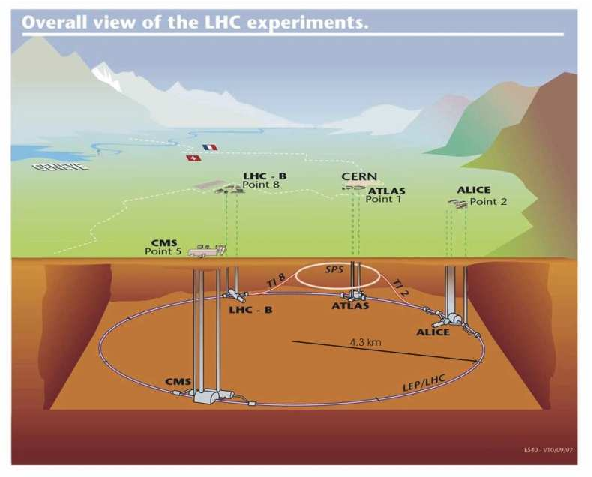
\includegraphics[height = 6.5cm]{top_view_lhc}
\caption[Vista aérea do LHC.]{Vista aérea do LHC (extraído de \cite{bib:site_lhc}).}
\label{fig:vista_aerea_lhc}
\end{center}
\end{figure}

Como os feixes de prótons trafegam por tubos separados, para colidi-los é feito o seguinte: em pontos específicos do acelerador, chamados de ``pontos de colisão'', não existem campos magnéticos, de forma que, nestas regiões, os feixes percorrem uma trajetória retilínea. Desta maneira, os dois feixes podem ser reunidos em um ambiente a vácuo e postos, finalmente, em rota de colisão.

Os prótons são inseridos no acelerador em rajadas de uns poucos centímetros de comprimento e alguns micrômetros de raio. A distância entre uma rajada e outra é de 7,5 metros. Uma vez que a luz demora 25 nanosegundos para percorrer 7,5 metros, e os prótons estão praticamente se movendo à velocidade da luz, conclue-se que as rajadas irão cruzar-se (e os prótons colidirem) com uma freqüência de 40 MHz. Entretanto, o número de colisões entre prótons depende da quantidade de prótons em cada rajada, o tamanho dos mesmos e do desenho do acelerador. Para uma alta taxa de
colisões, deve-se ter rajadas de curto comprimento, muitos prótons por rajada e muitas rajadas por unidade de tempo. Estas propriedades, que dependem do projeto do acelerador, podem ser combinadas em um único parâmetro: \textbf{luminosidade}.

A luminosidade é definida como a constante de proporcionalidade entre a taxa de colisões entre prótons e a área do próton. Em física experimental de partículas, atingir níveis elevados de luminosidade é tão importante quanto atingir níveis elevados de energia. Isto ocorre porque nem todas as colisões produzem os mesmos efeitos, e os tipos de colisões que geram eventos de interesses são extremamente raros. Por isso, são necessárias muitas colisões distintas (ou seja, alta luminosidade) para que se aumente a probabilidade de observação de eventos de interesse. No LHC, espera-se, com a luminosidade de operação ($1 \times 10^{34}$ cm$^{-2}$ s$^{-1}$ \cite{bib:tdaq_tdr}), atingir um total de um bilhão de colisões por segundo, sendo que deste valor, apenas um número entre 10 e 100 colisões poderão vir a ser de potencial interesse científico. No caso do bóson de Higgs, dada a sua raridade, esta taxa pode cair para um valor tão baixo que serão necessárias horas, e até mesmo dias, para que um único decaimento deste tipo possa vir a ocorrer.

Entretanto, para que seja possível aos físicos realizar as análises necessárias nos eventos gerados durante a colisão, sistemas de detecção devem ser posicionados em torno dos pontos de colisão para realizar a captura dos eventos gerados, e convertê-los em informação interpretável para os físicos. Visando este fim, o LHC possui diversos detectores:

\begin{itemize}

\item \textbf{ATLAS (\emph{A Toroidal LHC Apparatus})} $\rightarrow$ Este experimento, composto por vários detectores, será capaz de, entre outras coisas, provar experimentalmente a existência do bóson de Higgs. Detalhes deste experimento serão vistos na seção \ref{SEC:ATLAS}.

\item \textbf{CMS (\emph{Compact Muon Solenoid})} $\rightarrow$ A maioria dos detectores em física de partículas estão posicionados em torno de dispositivos magnéticos, de forma a tornar possível medir o momento de partículas carregadas. Este experimento contará com um solenóide supercondutor capaz de gerar um campo magnético de 4T (cem mil vezes maior do que o campo magnético da Terra), permitindo que dispositivos de detecção de traços e calorimetria sejam inseridos dentro das espiras do solenóide gerador do campo magnético, resultando em um poderoso detector de uso geral, composto inclusive, por detectores de múons \cite{bib:cms}.

\item \textbf{LHCb (\emph{A High Energy Physics Experiment Studying CP Violation})} $\rightarrow$ Este experimento visa estudar a violação CP\footnote{No mundo atômico, cada elemento possui a sua imagem ``espelhada'' (neutrinos e anti-neutrinos, por exemplo), entretanto, a anti-matéria nem sempre se comporta como uma imagem espelhada da matéria, de tal forma que a este fenômeno dá-se o nome de violação CP.}. Com o detector sendo desenvolvido neste experimento, os físicos serão capazes de detectar minúsculas diferenças entre matéria e anti-matéria \cite{bib:lhcb}.

\item \textbf{ALICE (\emph{A Large Ion Collider Experiment})} $\rightarrow$ O projeto ALICE consiste em um detector dedicado de íons pesados que explorará as interações entre núcleos atômicos ocorridas à energias elevadas, como as fornecidas pelo LHC. O objetivo é estudar a física de matérias fortemente interativas à densidades de energia elevadíssimas, onde se espera a formação de uma nova fase da matéria: o plasma quark-glúon \cite{bib:alice}.

\item \textbf{TOTEM (\emph{Total Cross Section, Elastic Scattering
and Diffraction Dissociation})} $\rightarrow$ Este experimento é dedicado a medir a seção transversal total, dispersão elástica e processos difrativos no LHC. Com isso, espera-se fornecer uma calibração exata da luminosidade do LHC \cite{bib:totem}.

\end{itemize}



\section{O Detector ATLAS (\emph{A Toroidal LHC Apparatus})}
\label{SEC:ATLAS}

\begin{figure}
\begin{center}
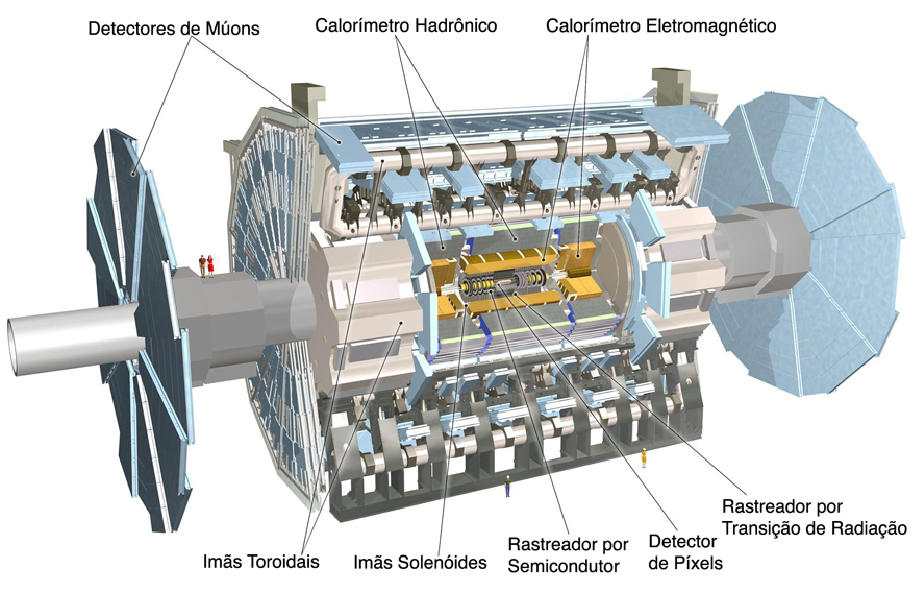
\includegraphics[height = 7cm]{atlas_detector}
\caption[Diagrama ilustrativo do detector ATLAS.]{Diagrama ilustrativo do detector ATLAS (extraído de \cite{bib:atlas}).}
\label{FIG:DETECTOR_ATLAS}
\end{center}
\end{figure}

Quando prótons colidem, alguns dos eventos gerados podem trazer informações relevantes ao experimento, enquanto que muitas outras colisões ordinárias (que não trazem nenhuma informação nova, e por isso, são comumente tratadas como ruído de fundo da experiência) são adquiridas. Assim, uma das principais necessidades de experimentos realizados com aceleradores de partículas é a separação dos eventos de interesse dos eventos de física ordinária. A diferenciação entre eventos é baseada nos produtos observados em cada colisão: energia, direção de movimento, etc. Para se identificar os eventos de interesse, torna-se necessário um poderoso detector que fornecerá informação detalhada sobre os produtos obtidos através das colisões realizadas no LHC. Este é o caso do detector ATLAS \cite{bib:site_atlas}. O projeto deste detector é o maior esforço colaborativo jamais visto na física, envolvendo 1800 cientistas de mais de 150 universidades em 34
países.

Observa-se, na Figura \ref{FIG:DETECTOR_ATLAS}, um diagrama ilustrativo do detector ATLAS, dando idéia de suas dimensões. Este detector está dividido em módulos distintos, conforme se pode analisar observando-se a seção transversal do mesmo, apresentada na Figura \ref{FIG:SECAO_TRANSVERSAL_ATLAS}, onde cada número indica um módulo específico, a saber:

\begin{figure}
\begin{center}
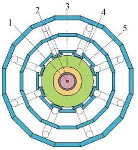
\includegraphics[height = 5.5cm]{atlas_detector_crossview}
\caption[Seção transversal do detector ATLAS.]{Seção transversal do detector ATLAS (extraído de \cite{bib:site_atlas}).}
\label{FIG:SECAO_TRANSVERSAL_ATLAS}
\end{center}
\end{figure}

\begin{enumerate}

\item \textbf{Tubo do Feixe:} o tubo do feixe passa através do centro do detector e carrega o feixe de prótons. Feixes viajando em sentido contrário através deste tubo são postos para colidir no meio do detector.

\item \textbf{Detector de Traços:} a região interna do detector está repleta de sensores altamente segmentados feitos de tiras de silício, de forma que a trajetória de partículas carregadas possa ser precisamente determinada. A trajetória de uma partícula carregada é curva, se a mesma estiver sob a influência de um campo magnético. O raio da curvatura e a direção da deflexão indicam, respectivamente, o momento e a carga da partícula.

\item \textbf{Calorímetro Eletromagnético:} este calorímetro consiste em finas pastilhas de chumbo (1,5 mm de espessura) separadas por sensores. Quando fótons ou elétrons de alta energia atravessam o chumbo (ou outro material de número atômico elevado), eles produzem um chuveiro eletromagnético\footnote{Um chuveiro eletromagnético ocorre quando um elétron (ou pósitron) é deflexionado pelo campo elétrico dos átomos, fazendo com que estes emitam fótons. Os fótons, por sua vez, geram elétrons (ou pósitrons), que por sua vez, geram mais fótons, e assim sucessivamente.}. O que acontece é que a energia inicial destas partículas é convertida em um grande número de elétrons e pósitrons de mais baixa energia, mas ainda em alta velocidade. O número final de elétrons / pósitrons é proporcional à energia da partícula incidente. 

As pastilhas de chumbo estão imersas em um tanque de argônio líquido. As reentrâncias (aproximadamente 4 mm), preenchidas com argônio líquido entre as pastilhas, estão sujeitas a um forte campo elétrico. Quando um chuveiro de elétrons, produzido dentro do chumbo, chega ao argônio, ele gera um rastro de pares elétrons-íons ao longo do seu caminho \cite{bib:knoll_radiation_detection}. O campo elétrico, então, faz com que os elétrons migrem para o lado positivo (muito mais rapidamente do que os íons migram para o lado negativo), gerando uma corrente elétrica em um circuito externo conectado ao calorímetro. Quanto maior a energia incidente, maior o número de chuveiros de elétrons e, conseqüentemente, maior a corrente gerada.

Este calorímetro está dividido em quatro camadas sobrepostas, com espessuras específicas, onde a terceira camada é a mais espessa. Além disso, cada camada possui granularidade específica, o que ajuda a determinar alguns aspectos dos objetos que interagem com este detector \cite{bib:msc_rabello}. Por fim, visando a redução de custos, a granularidade varia dentro de uma mesma camada, sendo menor (menor resolução) nas bordas do detector, regiões onde o aparecimento de eventos de interesse serão mais raros.

As conexões elétricas com o calorímetro são feitas, de fato, a finos membros metálicos imersos em argônio líquido (eletrodos). Estes eletrodos são subdivididos em pequenas regiões retangulares. Tais regiões, a várias profundidades, são agrupadas e unidas para formar camadas, de tal forma que, quando uma partícula atinge este calorímetro, tem-se a informação da energia depositada através de várias camadas, aumentando a resolução da detecção, uma vez que se adiciona mais uma dimensão de observação da interação de partículas com este calorímetro.

\item \textbf{Calorímetro Hadrônico:} este dispositivo mede a energia dos hadrons que o atingem, incluindo prótons, nêutrons, píons e káons (elétrons e fótons foram absorvidos na seção eletromagnética). O calorímetro hadrônico consiste em absorvedores metálicos separados por telhas de material cintilante. A interação de hadrons de alta energia com os absorvedores transformam a energia incidente em um chuveiro hadrônico, constituído por vários prótons e nêutrons de baixa energia, e outros hadrons. Este chuveiro, quando atravessa o material cintilante, faz com que este emita luz, em quantidade proporcional à energia incidente. Entretanto, uma vez que os hadrons podem iniciar seus chuveiros no calorímetro eletromagnético, os sinais obtido pelos dois calorímetros precisam ser somados para se obter a energia hadrônica total. Tal como o calorímetro eletromagnético, o calorímetro hadrônico também está dividido em camadas, possuindo, neste caso, três camadas sobrepostas, de forma a acrescentar mais uma dimensão de observação da deposição de energia.

A energia total emanada do ponto de colisão é menos intensa para grandes angulações (próximo a 90 graus), e mais intensa a ângulos menores em relação ao feixe. Devido ao fato que as telhas cintilantes podem se danificar se expostas à radiação, a calorimetria hadrônica, para ângulos entre 5 e 25 graus, é fornecida por um dispositivo de argônio muito similar ao utilizado no calorímetro eletromagnético. As principais diferenças são que as pastilhas de chumbo são substituídas por pastilhas de cobre (com espessura de 2,5 cm), que são mais apropriadas para o chuveiro hadrônico, e as reentrâncias entre as pastilhas distam 8 mm uma das outras.

\begin{figure}
\begin{center}
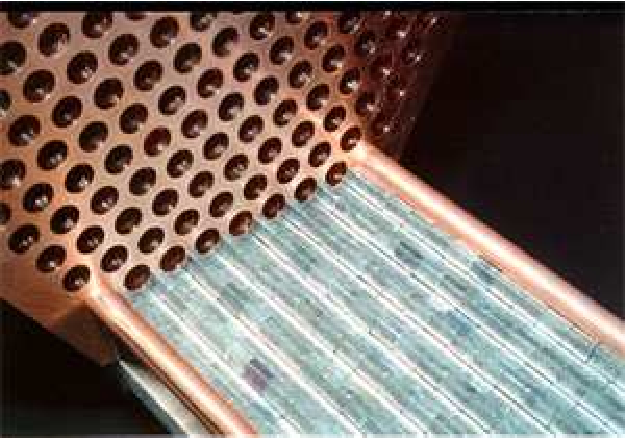
\includegraphics[height = 5cm]{hadron_forward}
\caption[Ilustração das barras metálicas sendo inseridas nos tubos da calorímetro de argônio líquido do calorímetro hadrônico.]{Ilustração das barras metálicas sendo inseridas nos tubos da calorímetro de argônio líquido do calorímetro hadrônico (extraído de \cite{bib:site_atlas}).}
\label{FIG:BARRAS_CALORIMETRO_HADRONICO}
\end{center}
\end{figure}

Para permitir a cobertura angular total, é necessário estender o calorímetro para que este detecte jatos a ângulos tão pequenos quanto 1 grau relativo aos feixes. Devido ao ambiente extremamente radioativo na região angular entre um e cinco graus, a calorimetria precisa ser desenvolvida com cuidados especiais. Nesta região, o calorímetro de argônio líquido tem suas pastilhas metálicas substituídas por uma matriz metálica que contém tubos ocos embutidos, de diâmetro interno de 5 mm. Barras metálicas de 4,5 mm são posicionadas dentro destes tubos (vide Figura \ref{FIG:BARRAS_CALORIMETRO_HADRONICO}), e o argônio líquido preenche o pequeno espaço existente entre as barras e os tubos que as contém. Algumas centenas de volts entre uma barra e um tubo produzem o campo elétrico necessário para fazer os elétrons migrarem dentro do argônio líquido, após a ionização gerada pelo chuveiro hadrônico.


\item \textbf{Detector de Múons:} múons interagem com qualquer partícula carregada. Entretanto, como são cerca de 200 vezes mais pesados do que elétrons, estas partículas são muito menos afetadas pelo campo elétrico dos átomos que estejam no caminho desta partícula. Desta forma, múons não geram chuveiros eletromagnéticos, dissipando pouca energia, e somente através da ionização de átomos que estejam em seu caminho. Assim, qualquer partícula energética que chegue a este detector é classificada como múon ou neutrino, visto que as demais partículas foram totalmente absorvidas pelos calorímetros. Entretanto, neutrinos também não interagem com este detector, escapando do mesmo. A presença de neutrinos, desta forma, só pode ser inferida pela energia que sobra do processo.

\end{enumerate}

Cada módulo observará um conjunto específico de propriedades das partículas. Estes módulos são empilhados de tal forma que as partículas possam percorrem todas as camadas seqüencialmente. Uma partícula não se tornará visível até que interaja com uma ou mais camadas do detector, ou que se decomponha em partículas que o façam. Pode-se visualizar, na Figura \ref{FIG:INTERACAO_PARTICULAS_ATLAS}, um exemplo de interação de diversas partículas com as diferentes camadas (módulos) do detector. Como se pode observar, partículas carregadas, como prótons e elétrons, são detectadas tanto na câmara de traços, bem como no calorímetro eletromagnético. Partículas neutras, como nêutrons e fótons, não são detectadas na câmara de traços, só sendo observadas quando interagem com outras camadas do detector. Fótons são detectados somente no calorímetro eletromagnético, enquanto que nêutrons são detectados somente no calorímetro hadrônico. Ou seja, cada partícula deixa a sua própria assinatura, ao interagir com um ou mais módulos do detector. 

\begin{figure}
\begin{center}
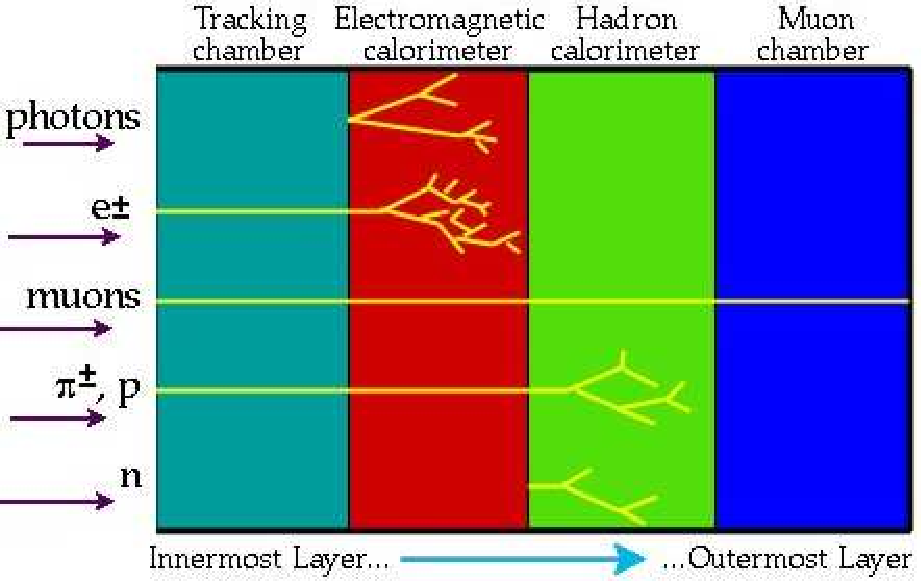
\includegraphics[height = 5.5cm]{decay_chart}
\caption[Interação de diferentes partículas com os diversos módulos do detector ATLAS.]{Interação de diferentes partículas com os diversos módulos do detector ATLAS (extraído de \cite{bib:site_atlas}).}
\label{FIG:INTERACAO_PARTICULAS_ATLAS}
\end{center}
\end{figure}


Espera-se, para este detector, que cada evento gere aproximadamente 1 Mbyte de informação, mas como a taxa de geração de eventos é de 40 MHz, o fluxo de dados será da ordem de 40 TBytes por segundo, o que é um valor impossível de ser armazenado para processamento \emph{offline}, uma vez que o experimento será executado por vários dias. Além disso, pouquíssimos eventos serão de real interesse para o experimento, de tal maneira que um sistema de filtragem \emph{online} deve ser desenvolvido para selecionar somente os eventos de potencial interesse para o projeto, descartando os que não apresentem informação nova, reduzindo desta maneira, o fluxo de informação a ser armazenada para posterior análise.

\chapter{Sistema de Filtragem}
\label{chap:sistema_filtragem}

Como visto no capítulo \ref{chap:lhc}, um volume enorme de informação é gerado a cada colisão no LHC. Viu-se, também, que os eventos de possível interesse para a detecção do bóson de Higgs, ou dos demais canais físicos de interesse, ocorrem com um período que varia de algumas horas a até dias de operação. Como cada evento, ao interagir com os detectores do ATLAS, produz aproximadamente 1,5 Mbyte de informação, e espera-se uma taxa de 40 MHz de eventos sendo gerados pelo LHC, o fluxo de dados será da ordem de 60 TBytes por segundo \cite{bib:tdaq_tdr}, impossibilitando o armazenamento completo desses eventos para análise \emph{offline}. Desta maneira, um sistema de filtragem \emph{online} \cite{bib:real_time_processing} torna-se indispensável para o experimento. O sistema de filtragem deverá identificar os padrões de decaimento do Higgs, e demais eventos de interesse, para poder localizá-los na massa de eventos com física ordinária, produzida pelas interações mal-sucedidas (interações que produzem canais físicos já conhecidos e que, portanto, significam ruído de fundo para o experimento).

O sistema de filtragem (\emph{trigger}) do ATLAS e o sistema de aquisição de dados é baseado em três níveis sequenciais de seleção \emph{online} de eventos. Partindo de uma taxa de eventos de 40 MHz, a taxa de eventos armazenados precisa ser reduzida, ao final do processo de seleção, para aproximadamente 100 Hz para armazenamento em base de dados e posterior análise \emph{offline}. Enquanto se requer uma alta taxa geral de rejeição, a eficiência na identificação dos eventos de interesse precisa ser elevada, de forma a ser capaz de reter eventos físicos raros \cite{bib:lvl1_trigger_tdr}.

\begin{figure}
\begin{center}
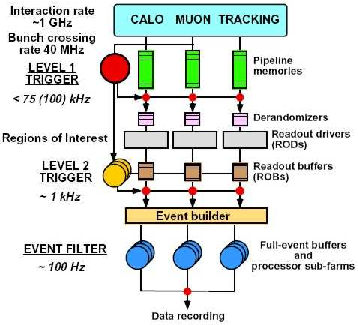
\includegraphics[height = 7.5cm]{block_diagram_trigger}
\caption{Diagrama em blocos do sistema de filtragem.}
\label{fig:block_diagram_trigger}
\end{center}
\end{figure}

Observa-se, na Figura \ref{fig:block_diagram_trigger}, o diagrama em blocos do sistema de \emph{trigger}. Como se percebe, o mesmo está dividido em três níveis principais de validação. A informação gerada pelos detectores é passada para o primeiro nível, que realiza a análise inicial, com granularidade reduzida. Os eventos aprovados pelo primeiro nível são armazenados em \emph{buffers} de leitura, para que possam ser acessados pelos níveis seguintes. O segundo nível opera somente sobre as regiões marcadas pelo primeiro nível, validando a decisão do mesmo, desta vez utilizando a granularidade total dos detectores. Em seguida, os eventos aprovados no segundo nível são enviados ao filtro de eventos (terceiro nível), onde a informação completa de cada evento é utilizada. Por fim, os eventos que são aprovados pelo filtro de eventos são enviados para armazenamento em disco para posterior análise \emph{offline}. Maiores detalhes sobre os três níveis de filtragem serão apresentados a seguir.


\section{Primeiro Nível de \emph{Trigger}}

O primeiro nível de \emph{trigger} (LVL1) realiza a seleção inicial, baseando-se na informação obtida com granularidade reduzida (baixa resolução) gerada por um sub-conjunto de detectores (calorímetros e câmara de múons). A granularidade neste nível é reduzida, uma vez que o tempo para a tomada de decisão neste nível é tão curto que torna-se necessário a redução da quantidade de informação a ser processada, para aumentar a velocidade de processamento. A redução da granularidade é produzida através do agrupamento das células dos calorímetros em conjuntos contendo 6 células, onde as céluas de cada conjunto são analogicamente somadas, produzindo um único sinal. Consequentemente,  este nível só descarta eventos com características bem distintas dos canais de interesse desejados. Múons de momento transverso ($P_T$) elevado são identificados usando apenas as chamadas câmaras de \emph{trigger}, câmaras de placas resistivas no barril, e câmaras de abertura fina nas beiradas \cite{bib:muon_spectrometer_tdr}. A seleção do calorímetro é baseada na informação com granularidade reduzida obtida dos calorímetros do eletromagnético e hadrônico \cite{bib:tdr_liquid_argon, bib:tile_calorimeter_tdr}.


Conforme discutido em \cite{bib:atlas_trigger_status_report}, a maioria das análises físicas que foram consideradas no ATLAS podem ser feitas, no primeiro nível, usando critérios de seleção relativamente simples. Entretanto, a implementação do primeiro nível é flexível e pode ser programada para selecionar eventos usando critérios mais elaborados.

\begin{table}
\centering
\footnotesize
\begin{tabular}{|l|c|}
\hline
\textbf{Evento de Interesse} & \textbf{Freqüência (kHz)}\\
\hline
Múon, $p_T$ $>$ 20 GeV & 4 \\
\hline
Par de múons, $p_T$ $>$ 6 GeV & 1 \\
\hline
Grupo único EM (eletromagnético) isolado, $E_T$ $>$ 30 GeV & 22 \\
\hline
Par de grupos EM isolados, $E_T$ (energia transversa) $>$ 20 GeV & 5 \\
\hline
Jato, $E_T$ $>$ 290 GeV & 0.2 \\
\hline
Três jatos, $E_T$ $>$ 130 GeV & 0.2 \\
\hline
Quatro jatos, $E_T$ $>$ 90 GeV & 0.2 \\
\hline
Jato, $E_T$ $>$ 100 GeV e perdendo $E_T$ (\emph{missing energy}) $>$ 100 GeV & 0.5 \\
\hline
Tau, $E_T$ $>$ 60 GeV e perdendo $E_T$ $>$ 60 GeV & 1 \\
\hline
Múon, $p_T$ $>$ 10 GeV e grupo EM isolado, $E_T$ $>$ 15 GeV & 0.4 \\
\hline
Outros eventos & 5 \\
\hline
\textbf{Total} & $\sim$40\\
\hline
\end{tabular}
\normalsize
\caption{Exemplo de freqüência de observação de eventos no primeiro nível, com luminosidade máxima ($L = 10^{34}$ cm$^{-2}$
s $^{-1}$)}
\label{tab:frequencia_eventos_lvl1}
\end{table}

A taxa máxima de saída do primeiro nível de filtragem está limitada em 75 kHz (podendo ser expandida para 100 kHz). Conforme pode-se concluir da Tabela \ref{tab:frequencia_eventos_lvl1}, as taxas estimadas dos eventos de interesse correspondem, no total, à metade do limite máximo de aceitabilidade do primeiro nível. Entretanto, devido a incertezas intrínsecas nos cálculos, esta margem de segurança não está superestimada \cite{bib:lvl1_trigger_tdr}.

Um requerimento básico para o primeiro nível é que este deve identificar unicamente colisões de interesse. Dado o pequeno (25 ns) intervalo de tempo entre choques de dois pacotes de prótons, esta é uma consideração não trivial. No caso dos calorímetros, por exemplo, um desafio considerável a ser vencido é que o formato do pulso gerado por estes dispositivos pode se estender por várias colisões (efeito de \emph{pile-up} \cite{bib:knoll_radiation_detection}).

É importante que se mantenha o tempo de latência (tempo para formar e distribuir a decisão do filtro) no valor mais baixo possível. Durante este tempo, a informação de todos os canais do detector precisa ser retida em memórias do tipo \emph{pipeline}. Estas memórias estão geralmente contidas em circuitos integrados, posicionadas próximas ou junto ao detector, freqüentemente em regiões inacessíveis e imersas em ambientes de forte radiação. A latência do primeiro nível, medida do instante de uma colisão próton-próton até a decisão do primeiro nível estar disponível para o nível seguinte, deve ser menor que 2,5 $\mu$s. De forma a atingir esta exigência, o primeiro nível de \emph{trigger} está sendo implementado em \emph{hardware} de baixa programabilidade do tipo FPGAs (\emph{Field Programmable Gate Array}) \cite{bib:fpga}, devido à sua velocidade. O tempo de latência desejado para este nível de \emph{trigger} foi, então, estipulado para 2 $\mu$s, deixando 500 ns de margem de segurança \cite{bib:lvl1_trigger_tdr}.

Os eventos selecionados recebem uma etiqueta do LVL1 com a identificação do canal físico ao qual pertencem, e em seguida são lidos dos \emph{drivers} de saída dos detectores (\emph{Read Out Drivers} - ROD) e propagados para os \emph{Readout Buffers} (ROB) através dos cabos de leitura (\emph{Read Out Links} - ROL), ficando, assim, disponíveis como fragmentos de informação (vide Seção~\ref{sec:eformat}) para o sistema de filtragem de alto nível.\footnote{A parte de alto nível do sistema de \emph{trigger} corresponde ao segundo e terceiro nível, visto que são desenvolvidos em \emph{software} e executados em computadores de uso geral.}. Entretanto, de forma a reduzir o volume de tráfego de dados para o segundo nível, e, conseqüentemente, aumentar a banda passante entre estes dois níveis, o primeiro nível já marca as regiões de interesse (\emph{Region of Interest} - RoI), que correspondem a regiões do detector onde houve a incidência de algum evento, e que foi aceito pelo primeiro nível, de tal maneira que o segundo nível observará somente estas regiões de interesse, e não toda a área do detector.




\section{O Sistema de Filtragem de Alto Nível}
\label{sec:htl}

\begin{figure}
\begin{center}
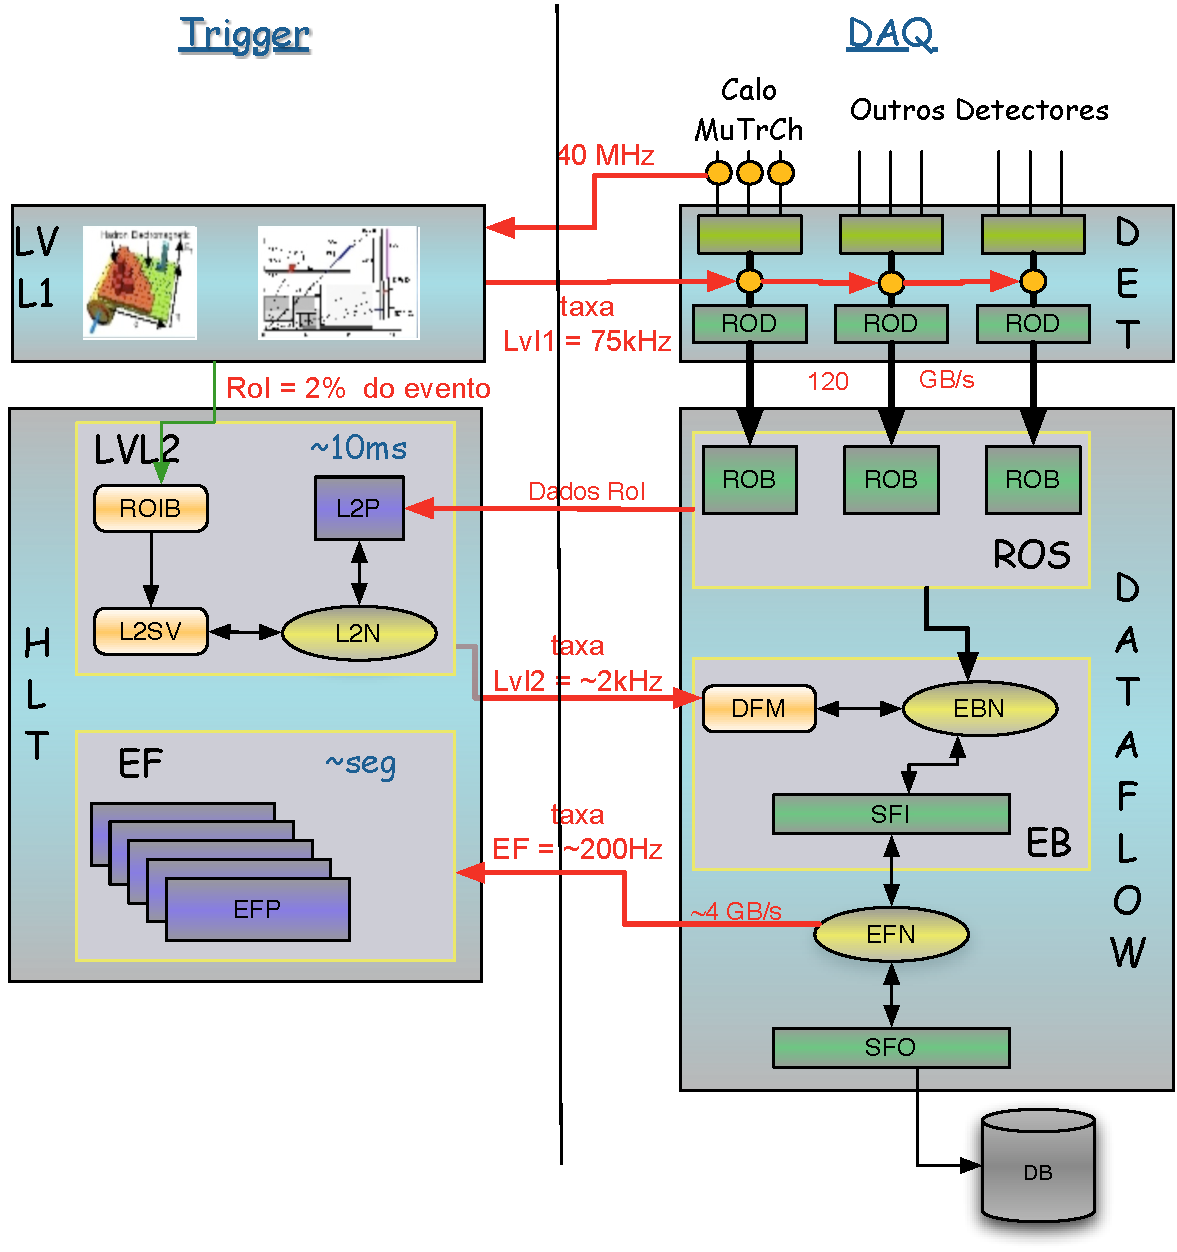
\includegraphics[height = 10cm]{tdaq_diagram}
\caption{Diagrama detalhado em blocos do sistema de filtragem de alto nível.}
\label{fig:tdaq_diagram}
\end{center}
\end{figure}

O sistema de filtragem de alto nível do ATLAS (\emph{High Level Trigger} - HLT) é composto pelo segundo nível \emph{LVL2} e pelo filtro de eventos (\emph{Event Filter - EF}), por serem todos implementados em \emph{software} com linguagem de programação de alto nível. A Figura~\ref{fig:tdaq_diagram} apresenta os detalhes desta parte do sistema de filtragem. Após a filtragem do LVL1, os eventos aprovados ficam disponíveis na forma de fragmentos nos sistemas de leitura (\emph{Read-Out Systems - ROS}). Além disso, a informação à respeito das RoIs etiquetadas pelo LVL1 são enviadas para o  construtor de RoI (\emph{RoI Builder} - RoIB). Este agrupa os fragmentos de informação gerados pelos diferentes detectores do ATLAS, e transmite o registro gerado por este agrupamento para um supervisor do segundo nível (\emph{LVL2 Supervisor - L2SV}) que ficará responsável por atribuir a uma unidade de processamento do segundo nível  (\emph{LVL2 Processing Unit} - L2PU) a RoI recebida. A L2PU então valida a etiqueta do LVL1, usando a granularidade total dos detectores, e retorna o resultado para o L2SV. Este envia o resultado para o gerenciador de fluxo de dados (\emph{Dataflow Manager - DFM}), para que o evento seja apagado em caso de rejeição, ou propagado para o filltro de eventos, caso sejam aprovados.  O DFM seleciona um dos processadores da fazenda de entrada (\emph{Sub-Farm Intut - SFI}) para que o mesmo solicite aos ROS toda a informação disponível do evento em questão. Uma vez a informação disponível, o SFI seleciona um dos processadores do filtro de eventos (\emph{EF Processor - EFP}), para que o mesmo realize analises detalhadas, usando toda a informação disponível para cada evento, e gerando, assim, a decisão final do sistema de filtragem. Os eventos finalmente aprovados são enviados às fazendas de saída (\emph{Sub-Farm Outtut - SFO}) para que possam ser armazenados em mídia permanente, para posterior análise \emph{offline}. A Tab.~\ref{tab:hlt_comp} apresenta o número de processadores necessários para cada módulo do sistema de filtragem de alto nível do ATLAS, considerando máquinas com 4 núcleos de processamento com \emph{clock} de 3 GHz cada.

Todo o segundo nível de filtragem foi desenvolvido utilizando, o máximo possível, tecnologias padronizadas (comerciais) \cite{bib:paper_lvl2}, visando fácil reposição de material e implementação simplificada. Todos os processadores são de uso geral (tipo PC) e praticamente todas as comunicações entre estes dispositivos são feitas através de \emph{switchs} Gigabit Ethernet, devido à velocidade, confiabilidade e padronização do protocolo. Todas as aplicações também estão desenvolvidas utilizando técnicas de orientação a objetos e implementadas em C++ \cite{bib:herbert_schildt_c++}.

\begin{table}
\begin{center}
\begin{tabular}{|l|c|}
\hline
Módulo & N$^o$ Processadores \\
\hline
ROS & 225 \\
\hline 
RoIB & 1 \\
\hline 
L2SV & 50 \\
\hline 
L2PU & 500 \\
\hline 
DFM & 1 \\
\hline 
SFI & 120 \\
\hline 
EFP & 1600 \\
\hline 
SFO & 35 \\
\hline 
Controle & 90 \\
\hline
\end{tabular}
\end{center}
\caption{Quantidade de processadores necessários para cada módulo do sistema de filtragem de alto nível do ATLAS.}
\label{tab:hlt_comp}
\end{table}

O sistema de filtragem de alto nível está dividido em duas partes: a aquisição e controle de dados e a parte de processamento dos eventos produzidos pelo ATLAS. Ambas descritas a seguir.

\subsection{Aquisição e Controle de Dados (\emph{Data Aquisition and Control - DAQ})}
\label{sec:daq} 

O DAQ é responsável pela propagação dos eventos pelo sistema de filtragem de alto nível do ATLAS. É responsabilidade de seus módulos garantir a integridade e correto fluxo da informação por todo o sistema. Além disso, o DAQ precisa assegurar que a informação chegará em tempo hábil, para atender os restritos requisitos de tempo. Por fim, o DAQ também é responsável por prover mecanismos de monitoração dos seus módulos, de forma a assegurar que os mesmos estejam funcionando corretamente. A seguir, serão apresentados os módulos que compõem o DAQ. 

\subsubsection{Sistemas de Leitura (\emph{Read-Out Systems - ROS})}
\label{sec:ros}

Os ROS são computadores de uso geral, tipo PC, que servem de interface entre o sistema de filtragem de alto nível e os eventos aprovados pelo LVL1. O ROS possui 3 componentes rincipais: o \emph{Buffer} de Leitura (\emph{Read-Out Buffer} - ROB), o \emph{IOManager} e o \emph{Controlador Local} .

O ROB provê armazenamento temporário dos fragmentos de informação produzidos por um dado ROD, para que sejam acessados pelo LVL2 e pelo Construtor de Eventos. Consequentemente, o ROB receberá fragmentos na taxa do LVL1, ou seja, 100 kHz. Todos os fragmentos de informação vindo de um ROD ficam armazenados pelo tempo de latência do LVL2, e aproximadamente 3\% destes, durante o tempo da construção do evento pelo Construtor de Eventos. Cada ROS possui 12 ROB, e cada ROB fica conectado a um único ROD através de um ROL. Para o tráfego dos fragmentos de informação com o sistema de filtragem, é utilizado uma rede gigabit ethernet dedicada para os dados do LVL2, e outra para os dados do Construtor de Eventos, de forma a diminuir o tempo de espera por fragmentos de informação. 

O \emph{IOManager} processa os requisitos de dados oriundos das L2PU e dos SFI. De acordo com o critério especificado na requisição do dado, o \emph{IOManager} coleta um ou mais fragmentos de ROB de um ou mais ROB, gera um fragmento de ROS (vide Seção~\ref{sec:eformat}) contendo os fragmentos de ROB selecionados, e envia este fragmento para o componente solicitante. O \emph{IOManager} também recebe do DFM requisições para liberar o espaço utilizado por fragmentos de ROB que já foram utilizados e devem ser apagados. Para otimizar a performance global do ROS, o \emph{IOManager} permite transmissões simultâneas de dados, isto é possível graças à arquitetura \emph{multi-thread} adotada no design deste componente.

 O Controlador Local prôve a interface entre o ROS e o software \emph{online}. Ele configura, controla e monitora todos os componentes dentro do ROS. A monitoração compreende tanto a monitoração operacional (tamanho de filas, páginas de memória utilizada, etc), e a provisão de amostras dos fragmentos de informação fluindo pelo ROS, com o objetivo de monitorar os detectores. O Controlador Local comunica-se com o software \emph{online} através da rede de controle, de tal forma a não impactar na velocidade de transmissão de fragmentos de informação do ROS.


\subsubsection{Geradores de Regiões de Interesse (\emph{RoI Builders - RoIB})}
\label{sec:roib}

Para cada evento aceito, o primeiro nível envia informações como a posição da RoI e valores de limiar alcançados. O RoIB combina estes fragmentos em um único registro que é passado a um L2SV. No esquema básico, cada L2SV verá apenas um subconjunto de L2P, de tal forma que a escolha do L2SV afeta o balanço de carga entre os L2P. O critério de seleção de L2SV utilizado pelo RoIB é o \emph{round-robin} \cite{bib:modern_operating_systems}.


\subsubsection{Supervisor do Segundo Nível (\emph{LVL2 Supervisor - L2SV})}
\label{sec:l2sv}

Os supervisores do segundo nível (L2SV) são um pequeno grupo de 50 processadores que supervisionam o fluxo de eventos no segundo nível e atuam como mediadores entre os sistemas do primeiro e do segundo nível. De forma a simplificar o gerenciamento dos processadores, os processadores utilizados para este fim serão de tipo similar aos que serão utilizados para a seleção de eventos. Entretanto, cada processador supervisor precisa de uma interface para receber dados do RoIB \cite{bib:tdaq_tdr}.

\begin{figure}
\begin{center}
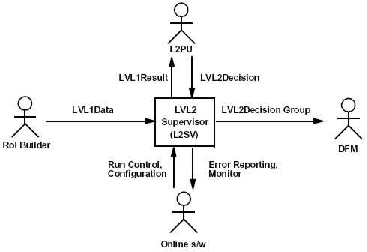
\includegraphics[height = 6cm]{lvl2_supervisor}
\caption{Contexto do supervisor do segundo nível.}
\label{fig:l2sv}
\end{center}
\end{figure}

O contexto do supervisor do L2SV é indicado na Figura \ref{fig:l2sv}. O L2SV recebe do RoIB a informação do primeiro nível em um único registro. O supervisor seleciona, então, um L2P para o evento e passa para uma das unidades de processamento (L2PU)\footnote{Um L2P pode ter várias L2PUs sendo executadas simultaneamente, visando maximizar a eficiência de uso da CPU.} o dado do primeiro nível. Uma vez que o algoritmo foi executado e uma decisão quanto ao evento foi tomada, a mensagem de decisão é passada para o L2SV. O Resultado é propagado, então, para o controlador de fluxo de dados (\emph{Data Flow Manager} - DFM) e para o L2HR. 

Ao selecionar um L2P, o supervisor o faz através de uma função de balanceamento de carga, examinando o numero de eventos na fila e associe cada evento ao processador menos carregado \cite{bib:tdaq_tdr}.


\subsubsection{Processadores do Segundo Nível (\emph{LVL2 Processors} - L2P)}
\label{sec:l2p}

O algoritmo de seleção do segundo nível é executado em uma rede de processadores do tipo PC com múltiplos núcleos de processamento. O tempo total de decisão médio, para cada evento do segundo nível, é de aproximadamente 10 ms. Entretanto, haverá uma larga variação entre os tempos gastos com cada evento, uma vez que certos eventos podem ser descartados logo no início do processo de seleção do segundo nível, enquanto que outros terão que ser propagados até o fim, para que uma decisão possa ser tomada. Cada evento será manipulado por um único processador, que requisitará dados aos ROS de cada RoI somente quando solicitado pelo algoritmo. Para manter uma alta eficiência de utilização de cada processador, enquanto este espera por um evento, vários eventos estarão sendo processados em paralelo dentro de um mesmo processador, tanto através da execução de várias cópias do \emph{software} de seleção, bem como pelo uso de múltiplas \emph{threads} dentro de um mesmo programa.

O processamento é executado em um único aplicativo rodando em cada processador. Este aplicativo contém três componente principais: a unidade de processamento do segundo nível (\emph{LVL2 Processing Unit} - L2PU), a interface de comunicação PESA (\emph{PESA Steering Controller} - PSC) e o \emph{software} de seleção de eventos (\emph{Events Selection Software} - ESS). A L2PU lida com o fluxo de dados com outras partes do sistema de \emph{trigger}, incluindo envio de mensagens, configuração, controle e supervisionamento. A PSC é executada dentro da L2PU e provê o ambiente e serviços necessários para o ESS. Como a L2PU controla a comunicação com o L2SV e os ROS, algumas interfaces precisam ser providas para as várias mensagens entre a L2PU e o ESS. A PSC provê a interface para o resultado do primeiro nível e retorna o resultado do segundo nível. Maiores detalhes sobre o ESS estão apresentados na Seção \ref{sec:offline}.

O desenvolvimento e implementação das L2PUs são baseados em um ambiente \cite{bib:tdaq_tdr} do qual são utilizados os seguintes serviços: controle, inicialização e configuração de aplicativos, relatório de erros, monitoração e envio de mensagens de aplicativos e instrumentação (este último para avaliação de performance).

As L2PU se comunicam com os supervisores do segundo nível, dos quais a mesma recebe a informação da RoI (gerada pelo primeiro nível) e para os quais ela retorna a decisão do segundo nível. Os dados da RoI (provenientes de vários ROB) são requisitados dos ROS, de acordo com a necessidade dos algoritmos de seleção.

Os algoritmos de seleção propriamente ditos são executados dentro de uma das \emph{threads} de execução (\emph{Worker Threads}), cada uma processando um evento. Esta abordagem \emph{multi-thread} foi adotada para evitar a parada da CPU enquanto a mesma aguarda pelo dado solicitado ao ROS. Este recurso também permite o uso eficiente de processadores contendo múltiplas CPUs, mas requer que o algoritmo de seleção de eventos seja seguro, no que diz respeito a esta implementação. Alguns serviços assíncronos (monitoração de aplicativos, entrada de dados) também são executados em \emph{threads} separadas.

\begin{figure}
\begin{center}
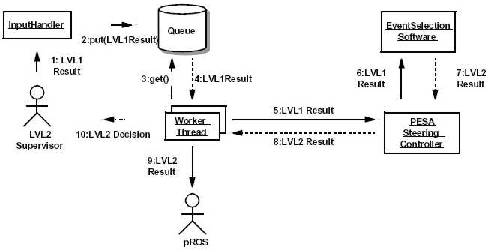
\includegraphics[height = 6cm]{eventsflow_lvl1_to_lvl2}
\caption{Fluxo de eventos aplicados a cada evento recebido do primeiro nível e que leva à decisão do segundo nível.}
\label{fig:app_l2p}
\end{center}
\end{figure}

Pode-se observar, na Figura \ref{fig:app_l2p}, o que acontece para cada evento no LVL2. O supervisor do segundo nível seleciona uma L2PU e envia o resultado do primeiro nível. Esta L2PU armazena o resultado recebido em uma fila compartilhada. Quando uma \emph{thread} fica disponível, a mesma retira da fila um evento, inicia o processamento do mesmo e produz, ao final, o resultado do segundo nível. Finalmente, a decisão do segundo nível é gerada a partir do resultado gerado pela \emph{thread} e retornado ao supervisor do segundo nível. Se o resultado for positivo, o resultado é enviado, também, para o L2RH.


Quando os algoritmos de seleção necessitam de dados dos ROBs, o fornecedor de dados do ROB é ativado e seu funcionamento pode ser observado na Figura \ref{fig:l2pu_dc}. O coletor de dados dos ROB cuida das requisições de envio para os ROS apropriados, espera até que todos os dados cheguem, monta os fragmentos de ROS recebidos em uma lista de fragmentos de ROB que são retornados ao chamador. Em \cite{bib:tdaq_tdr}, exames de performance relacionados à coleta de dados de RoIs pelos ROB foram executados e os resultados excederam, por uma larga margem, as especificações de I/O exigidas pelo projeto.

\begin{figure}
\begin{center}
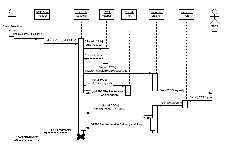
\includegraphics[width = 12cm]{l2pu_data_collection}
\caption{Coleta de dados dentro da lista de ROB (correspondentes a uma RoI) pela L2PU.}
\label{fig:l2pu_dc}
\end{center}
\end{figure}

Outro componente de destaque do L2P é a PSC. A PSC é o componente do sistema de \emph{trigger} de alto nível que realiza a interface entre a L2PU e o ESS. Os objetivos da PSC são três:

\begin{enumerate}

\item Permitir que a L2PU hospede e controle \emph{softwares} de seleção desenvolvidos \emph{offline}.

\item Permitir que os softwares de orientação possam ser compartilhados com o terceiro nível.

\item Prover um mecanismo para transmitir os resultados dos níveis 1 e 2 entre o sistema de fluxo de dados e o ESS.

\end{enumerate}

A chave do desenvolvimento da PSC é colocar esta interface onde a funcionalidade do fluxo de dados do segundo nível e o ESS podem ser perfeitamente separados. O local escolhido foi a máquina de estados finita da L2PU. A PSC provê os meios necessários para encaminhar mudanças no estado de controle de execução do software de fluxo de dados do segundo nível para o ESS, visto que o ESS está sendo desenvolvido no sistema \emph{offline} Athena (vide seção \ref{sec:offline}).


É apresentada, na Figura \ref{fig:l2pu_pesa}, a seqüência de interações da PSC entre a L2PU e o ESS. Na figura, pode-se observar três estados: 

\begin{enumerate}

\item \textbf{Configuração}: durante a fase de configuração, dados sobre condições e configurações são obtidos de uma base de dados externa, via interface \emph{online} do sistema de \emph{trigger}. Estes dados são, então, usados para configurar o ESS e todos os componentes associados.

\item \textbf{Início}: após o início, a PSC recebe uma diretiva de evento de execução, com um resultado do primeiro nível como argumento. A PSC, então, retorna (após execução do ESS) o resultado do segundo nível, direto à L2PU.

Um importante aspecto desta abordagem é que o manuseio de eventos do segundo nível é gerenciado inteiramente pelo pacote de coleta de dados. A PSC não precisa interagir diretamente com a \emph{thread} de entrada, o L2SV ou com o L2RH. As requisições por fragmentos de dados são ocultas, uma vez que são realizadas pelo serviço provedor de dados.

\item \textbf{Parada}: após a parada, a PSC termina a execução de algoritmos. Neste estágio, relatórios de execução podem ser produzidos para o processo de seleção.

\end{enumerate}


\begin{figure}
\begin{center}
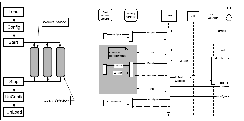
\includegraphics[height = 7.5cm]{l2pu_and_pesa_steering_controller}
\caption{A máquina de estados finita da L2PU (esquerda) e a interface PESA (direita).}
\label{fig:l2pu_pesa}
\end{center}
\end{figure}

\begin{figure}
\begin{center}
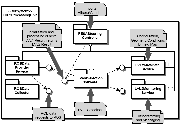
\includegraphics[height = 6cm]{dependencies_ess}
\caption{Dependências do ESS executando a seleção de eventos na L2PU.}
\label{fig:dependencies_ess}
\end{center}
\end{figure}

Pode-se observar, na Figura \ref{fig:dependencies_ess}, o diagrama para a execução do ESS na L2PU. A comunicação com sistemas externos e sub-sistemas, incluindo o L2SV e o ROS, estão ocultos do ESS. O ESS é inicializado conforme a Figura \ref{fig:l2pu_pesa}. O PSC fornece ao ESS os resultados do primeiro nível e requisita a seleção do segundo nível. Para fornecer o resultado do segundo nível, o ESS precisa acessar o serviço de fornecimento de dados do ROB. A requisição de dados ao ROB é enviada através do serviço de fornecimento de dados do ROB para o coletor de dados do ROB.


\subsubsection{Manipulador de Resultados do Segundo Nível (\emph{LVL2 Result Handler} - L2RH)}

Para todos os eventos aceitos pelo segundo nível, os detalhes do processamento deste nível (e o resultado completo do primeiro nível, recebido pelo supervisor) são fornecidos pela L2PU para que sejam incluídos ao evento. Entretanto, os ROS só armazenam dados provenientes do LVL1. Para resolver este problema, o L2RH foi desenvolvido. Este componente opera de maneira bastante similar ao ROS, só que recebe a informação gerada pelo LVL2. A informação do LVL2 é enviada via rede como um fragmento de ROB para o L2RH, onde é armazenada, enquanto aguarda sua requisição pelo construtor de eventos, que enxerga o L2RH como um ROS. Quando o evento é construído, o L2RH é inserido com todos os outros ROSs, de forma a incluir o resultado do segundo nível na construção do evento, que será enviado ao filtro de eventos. Uma única unidade como essa é suficiente para lidar com o volume de dados ao final do segundo nível, onde se espera um fluxo de uns poucos kilobytes por segundo, considerando uma taxa de aceitação de 3 kHz.


\subsubsection{Gerenciador de Fluxo de Dados (\emph{Dataflow Manager} - DFM)}

Este componente se encarrega de receber os resultados das decisões realizadas pelo LVL2. Eventos rejeitados são salvos em uma fila, de forma que, quando esta fila enche, o DFM dispara uma mensagem para todos os ROS solicitando que estes removam de seus ROB os fragmentos de informação pertencentes aos eventos rejeitados. Para os eventos aprovados, o DFM opera de maneira análoga ao L2SV. Ele seleciona um SFI menos carregado e envia a este as informações de um dado evento aprovado, para que este seja construído pelo SFI. Ao final da construção do evento, o DFM solicita aos ROS que apaguem os fragmentos de informações referentes a este evento, visto que durante a construção, estes fragmentos são copiados para o SFI, de forma a liberar espaço nos ROB. 


\subsubsection{Fazendas de Entrada (\emph{Subfarm Input} - SFI)}

O SFI é o dispositivo encarregado de requisitar e receber todos os fragmentos de dados de um determinado evento, para a que o mesmo seja montado e propagado ao filtro de eventos. Após a montagem do evento, o SFI informa ao DFM que o evento já foi corretamente montado, de forma que o DFM possa solicitar aos ROS que apaguem as informações referentes ao evento montado. Para aumentar a eficiência de utilização de um SFI, várias \emph{threads} operam concorrentemente, permitindo a construção de vários eventos em paralelo dentro de um mesmo SFI. O SFI também é responsável por enviar a um processador do filtro de eventos o evento totalmente construído. Somente após o processador do filtro de eventos acusar o correto recebimento do evento montado, o mesmo é apagado da memória do SFI \cite{bib:eb}.


\subsubsection{Processador do Filtro de Eventos (\emph{Event Filter Processors} - EFP)}

O EFP é o componente que solicitará ao SFI ao qual está conectado, um evento construído, para realizar a validação final sobre o mesmo. Cada EFP executa um programa de controle de fluxo de dados (\emph{Event Filter Dataflow} - EFD) que receberá dos SFI os eventos construídos. Adicionalmente, cada EFP possui várias Unidades de Processamento (\emph{Processing Tasks} - PT). As PT são encarregadas de processar os eventos recebidos pelo EFD. Enquanto a L2PU observa apenas parte do detector (RoI), a PT analisará toda a informação disponível para cada evento.  Quando uma dada PT completa o processamento de um evento, ela requisita um novo. Os dados gerados pela PT durante o processamento são anexados ao evento completo, caso tenha sido aceito pela PT. Os eventos aceitos são classificados e movidos para o respectivo SFO, para serem gravados em arquivos em disco.

Os EFP estão organizados em conjuntos, onde cada conjunto está associado a um ou mais SFI ou SFO. SFI, SFO e os EFP estão conectados através de um \emph{switch} Ethernet de alta velocidade (Gigabit Ethernet).


\subsubsection{Fazendas de Saída (\emph{Subfarm Output} - SFO)}

Após a validação final de cada evento pelas PT, os eventos aprovados devem ser finalmente  armazenados em mídia permanente para posterior análise \emph{offline}. Quando um EFD aprova um evento, ele o envia para o SFO, para que o mesmo o armazene em arquivos em disco. Estes arquivos são posteriormente acessados por um sistema de armazenamento em massa para armazenamento definitivo \cite{bib:tdaq_tdr}.


\subsubsection{Comunicação entre os Módulos do Sistema de Filtragem}

Para o transmissão de dados entre os módulos do sistema de filtragem de alto nível do ATLAS, utiliza-se \emph{switchs} Gigabit \emph{ethernet}. Para lidar com o enorme fluxo de informações, existem redes específicas para cada parte do sistema de filtragem de alto nível. A rede de controle (\emph{Control Network} - CTRLN) conecta todos os dispositivos. Informações de configuração, monitoração, notificações de erros são transmitidas por cada módulo utilizando esta rede. A rede de tráfego do segundo nível (\emph{LVL2 Network} - L2N) é responsável pelo tráfego de dados dos componentes pertencentes a este nível. Os L2SV enviam as informações sobre a RoI a ser validada para o L2P utilizando esta rede, e as L2PU requisitam aos ROS os fragmentos de informação necessários também utilizando esta rede. A L2N também conecta o L2SV com o DFM e o L2RH. A rede do contrutor de eventos (\emph{Event Bulder Network} - EBN) será utilizada para trafegar os dados a serem construídos entre os ROS, L2RH, DFM e SFI. Por fim, a rede do filtro de eventos (\emph{Event Filter Network} - EFN) conecta os EFP com os SFI e SFO. É apresentado na Figura~\ref{fig:net_design} o diagrama com a conexão das redes de tráfego de dados do sistema de filtragem de alto nível, para melhor visualização.

\begin{figure}
\begin{center}
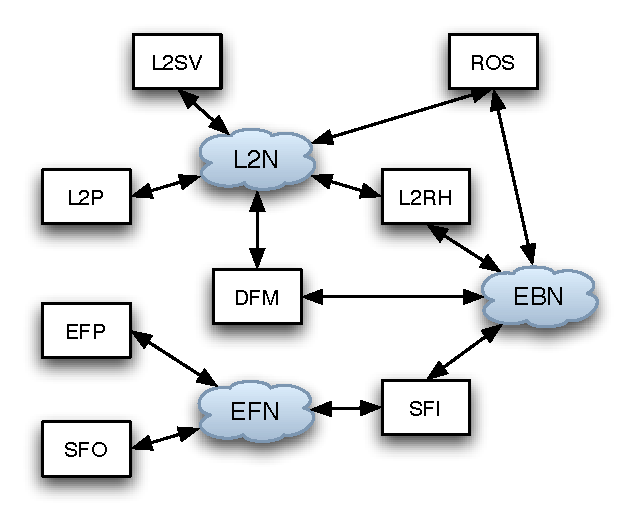
\includegraphics[height = 7cm]{hlt_network_design}
\caption{Diagrama de conexão das redes de dados do HLT.}
\label{fig:net_design}
\end{center}
\end{figure}


Como apresentado nesta seção, o volume de informação trafegando entre o LVL1 e o HLT é muito elevado. Além disso, o LVL1 opera próximo ao ATLAS, enquanto o HLT opera na superfície, separado do LVL1 por aproximadamente 200 metros. Consequentemente, a interface entre estas duas partes possuem alguns requisitos especiais, a saber:

\begin{itemize}

\item Palavra de 32 bits à 40,08 MHz ($\sim160$ Mbyte/s).

\item Resistência à radiação.

\item Latência muito pequena.

\item Comprimento máximo de 300 metros.

\end{itemize}

Estes requisitos tornam inviável a utilização de redes Gigabit \emph{ethernet}. Desta forma, os ROS e o RoIB estão conectados aos detectores do ATLAS por cabos de fibra óptica, usando protocolo de comunicação S-LINK \cite{bib:slink_spec}. O protocolo S-LINK é uma protocolo de comunicação ponto-a-ponto desenvolvido especialmente para atender os rígidos requisitos de transmissão entre o LVL1 e o HLT. Ao contrário de outros padrões, que definem a camada física de transmissão, o S-LINK define uma simples interface FIFO síncrona na qual os sinais de transmissão ficam independentes do canal físico. O mapeamento entre os sinais da S-LINK e do protocolo usado na camada física fica a critério do desenvolvedor do canal de transmissão, de forma que este pode realizar este mapeamento da forma mais adequada à tecnologia adotada no canal de transmissão.


\subsection{Athena}
\label{sec:offline}

O requisito básico exigido pelos físicos para realizarem suas tarefas é um conjunto de programas para realizar simulações de eventos, reconstruções, visualizações, etc. Além de um conjunto de ferramentas que permitam a escrita de programas de análises. Adicionalmente, os físicos desejam algo fácil de usar e extremamente flexível. Por fim, os físicos do ATLAS desejam desenvolver algoritmos de seleção de eventos para operarem \emph{online} no sistema de filtragem do ATLAS.

Para suprir estes requisitos, o Athena foi desenvolvido. O Athena é um \emph{framework} de controle que representa uma implementação concreta de uma arquitetura. A arquitetura por baixo do Athena é a arquitetura do Gaudi \cite{bib:gaudi}, originalmente desenvolvida para o LHCb. Esta arquitetura foi extendida através da colaboração com o ATLAS, e uma arquitetura base, desacoplada a um experimento específico, e também chamada Gaudi foi desenvolvida. O Athena é, então, a união desta arquitetura base com melhorias expecíficas ao ATLAS \cite{bib:athena_dev_guide}. 

O objetivo principal do Athena é isolar seus usuários de detalhes irrelevantes, como que tipo de biblioteca usar para transferência de dados, ou para gerar um gráfico. Para tal, sua arquitetura consiste na especificação de um número de componentes e suas interações entre si. Um componente é um bloco de código que possui uma funcionalidade e interface bem definida. Uma interface é uma coleção de métodos junto com uma descrição sobre o que cada método faz, ou seja, sua funcionalidade. Os principais benefícios desta abordagem são:

\begin{itemize}

\item \textbf{Flexibilidade}: esta abordagem provê simplicidade, dado que componentes podem ser conectados de diferentes maneiras para desempenhar diferentes tarefas.

\item \textbf{Simplicidade}: softwares para acessar, por exemplo, uma base de dados, são normalmente complexos de se aprender. Entretanto, a maioria dos detalhes são de pouco interesse para alguem que deseja simplesmente ler dados e salvar seus resultados. Desta forma, um componente para acessar dados pode ser desenvolvido de forma a fornecer somente a funcionalidade desejada. Além disso, a interface para este componente continuaria a mesma, independentemente da tecnologia de armazenamento utilizada pela base de dados do exemplo em questão. 

\item \textbf{Robustez}: como dito acima, um determinado componente pode ocultar de seu usuário a tecnologia que utiliza. Além de oferecer simplicidade, a vantagem que isto representa é que a tecnologia pode ser alterada sem que o usuário precise sequer saber desta mudança.

\end{itemize}


Alguns dos principais serviços e interfaces do Athena são:

\begin{itemize}

\item \textbf{Pythia}: o Athena provê interface para o Pythia. Este módulo é responsável por simular a colisão de feixes de partículas. 

\item \textbf{Geant}: o Geant é um conjunto de ferramentas que permitem simular a interação de partículas com a matéria. Desta forma, torna-se possível simular o comportamento dos detectores do ATLAS quando excitados por partículas. As simulações de Monte Carlo utilizadas para a análise e desenvolvimento de algoritmos de seleção são produzidas através da simulação de colisões geradas pelo Pythia, e a consequente descrição do comportamento dos detectores do ATLAS utilizando o Geant para descrever como estas partículas produzidas pelo Pythia interagem  com o material que compões dos detectores do ATLAS.  

\item \textbf{Storegate}: O Storegate é um amiente que permite a propagação de dados entre pacotes do Athena. Ele funciona como uma área de armazenamento, onde um dado algoritmo pode identificar e salvar informações geradas pelo mesmo no Storegate, de forma que os algoritmos subsequentes possam recuperá-lo, ao fornecer ao Storegate a chave de identificação do dado desejado.

\end{itemize}


Dado a flexibilidade do Athena, este está sendo utilizado para o desenvolvimento de algoritmos de seleção de eventos. Este algorimtos podem acessar as simulações de Monte Carlo que reproduzem a colisão de partículas e a consequente interação destas com os detectores do ATLAS para realizar processos de extração de características e tomadas de decisão. Muitos destes algoritmos  operam somente em modo \emph{offline}. Entretanto, como dito acima, o Athena também será usado na filtragem \emph{online} do ATLAS, de forma que uma famíilia especial de algoritmos foi desenvolvida para atender a este objetivo.

\subsubsection{Estratégia \emph{Online} para a Seleção de Eventos}

Como dito anteriormente, os eventos de interesse para o experimento ATLAS são bastante raros. Desta forma, lida-se com um volume muito maior de informação irrelevante, do que com eventos de interesse. Desta forma, a melhor estratégia de filtragem é rejeitar, o mais rápido possível, eventos considerados como ruído de fundo. A configuração e capacidades do sistema de filtragem de alto nível são dirigidas pela performance física (seleção de eventos e rejeição de ruído) e pela performance do sistema (velocidade de execução, requisitos de dados). O melhor compromisso entre estes fatores tem que ser encontrado de forma a maximizar a performance física. Para rejeitar eventos o mais rápido possível, uma abordagem de filtragem em etapas foi escolhida pelo ATLAS tanto para o LVL2, bem como para o EF. 

Para esta abordagem, um mecanismo de controle foi desenvolvido. Suas principais características são:

\begin{itemize}

\item Manter-se informado sobre quais algoritmos já foram executados para um dado evento, quais informações foram geradas por cada algoritmo e onde estas estão armazenadas. Adicionalmente, ele provê os mecanismos de persistência e propagação  da informação, e provê mecanismos de acesso à informação gerada por cada algoritmo.

\item Formar e manipular o resultado gerado para cada evento.

\item Acessar os resultados do LVL1 e do LVL2, que dará origem aos subsequentes passos de reconstrução.

\end{itemize}

No contexto deste controle, algumas entidades etão presentes:

\begin{itemize}

\item \textbf{Elemento de \emph{Trigger}}: entidade que é ativada por um determinado algoritmo para sinalizar a validação de um corte.  No LVL1, um elemento de \emph{trigger} é uma RoI. Já no sistema de filtragem de alto nível, eles são gerados através de sequências de algoritmos de extração de características e testes de hipótese.

\item \textbf{Assinatura}:  combinação de elementos de \emph{trigger} que podem levar a uma decisão positiva do sistema de filtragem. Os elementos de \emph{trigger} podem ser combinados por lógica booleana \texttt{AND}, \texttt{OR} e \texttt{NOT}. Adicionalmente a multiplicidade de elementos de \emph{trigger} pode ser configurada. Exemplo: uma assinatura  \texttt{e25i} representa um elétron isolado com energia transversa superior a 25 GeV. Já a assinatura \texttt{2e15i} é a assinatura produzida pelo sistema de filtragem quando dois elétrons isolados e com energia superior a 15 GeV são identificados.

\item \textbf{Menu}: consiste em uma série de assinaturas. Se uma ou mais assinaturas são satisfeitas, o evento é disparado.

\item \textbf{Cadeia}: sequência de algoritmos utiizados para ativar uma determinada assinatura.

\item \textbf{Slice}: um \emph{slice}  é a sequência de processamento utilizada para um tipo de partícula (elétron, fótons, múons, etc) e compreende os três níveis de filtragem (LVL1, LVL2 e EF).

\end{itemize}

É apresentado na figura~\ref{fig:athena_trigger_str} a organização do Athena no que tange a filtragem de alto nível do ATLAS. Podemos observar que um \emph{slice} compreende várias assinaturas contidas em um menu, onde cada uma delas é ativada por uma cadeia de algoritmos. Uma sequência pode ser composta por vários algoritmos de extração de características e de hipóteses. A combinação dos resultados de cada algoritmo de hipótese determinará se a assinatura será ativada ou não. A lista de assinaturas aprovadas e rejeitadas é inserida no \emph{TriggerDecision}, de forma que é possível saber, após a filtragem, quais assinaturas foram ou não aceitas.

\begin{figure}
\begin{center}
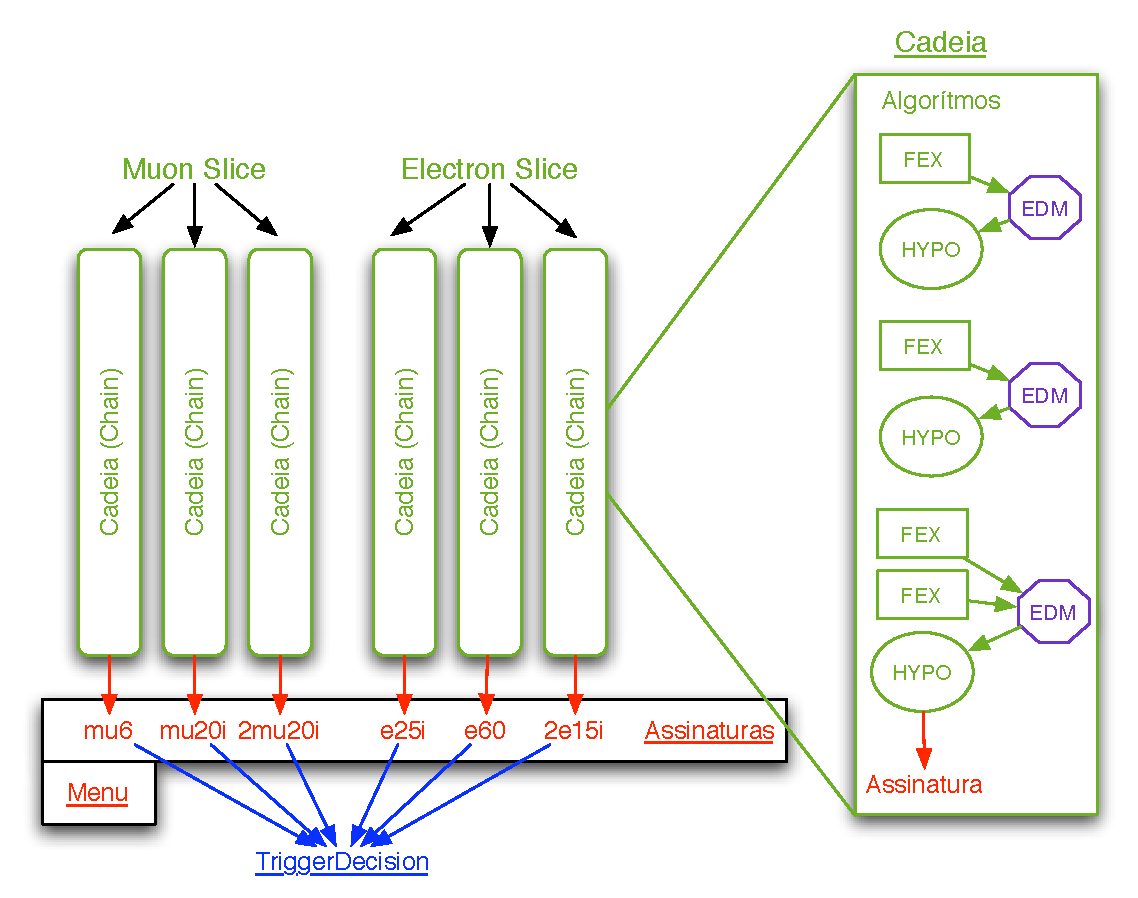
\includegraphics[height = 8cm]{athena_trigger_structure}
\caption{Organização do Athena para a filtragem de alto nível do ATLAS.}
\label{fig:athena_trigger_str}
\end{center}
\end{figure}

Para tornar o desenvolvimento de algoritmos para o sistema de filtragem independente do sistema de fluxo de dados, o Athena implementou camadas de abstração para a comunicação com a L2PU e a PT, de forma que é possível executar os algoritmos \emph{online} em ambiente \emph{offline}, para depois portá-los para o sistema de filtragem do ATLAS.

Durante a execução dos algoritmos de filtragem, é possível salvar em disco o resultado intermediário gerado por cada pacote em um arquivo chamado \emph{NTUPLE}, que pode ser aberto na ferramenta de análise ROOT \cite{bib:site_root} utilizada no CERN. Além disso, a geração de histogramas de qualquer variável de um dado algoritmo é possível, junto com histogramas com as informações de tempo de execução de uma dada parte do código. Tal como as \emph{NTUPLES}, os histogramas também podems er visualizados no ROOT.


\section{Fomatação dos Dados}
\label{sec:eformat}

A informação produzida pelos detectores do ATLAS precisa de uma formatação padronizada, de forma a facilitar a propagação e o processamento da mesma. Este formato deve atender aos seguintes requisitos:

\begin{itemize}

\item Tem que permitir que um evento cresça ou diminua, de acordo com configurações específicas do experimento.

\item Não pode ter uma limitação de tamanho para o evento.

\item Deve ser baseado em fragmentos, onde um fragmento, na sua apresentação mais baixa é o dado de um ROD.

\end{itemize}


Par atender estes requisitos, um formato chamado \emph{EFormat} foi desenvolvido \cite{bib:eformat}. O \emph{EFormat} define a estrutura do dado dentro dos vários estágios do sistema de filtragem de alto nível e do sistema de fluxo de dados. O formato também permite que dados adicionais sejam inseridos, pelo sistema de filtragem, aos dados provenientes do detector, permitindo que porcessos possam identificar rapidamente o tipo e a origem de um evento.

\begin{figure}
\begin{center}
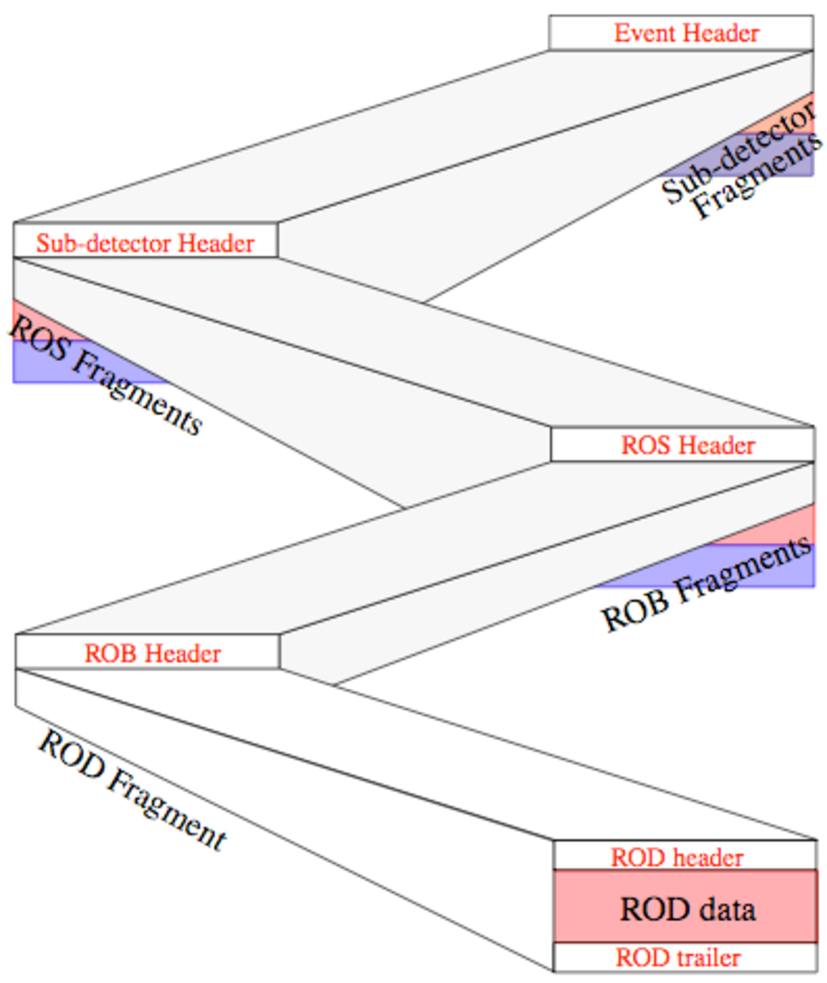
\includegraphics[height = 8cm]{eformat_structure}
\caption{Formato geral dos eventos propagados elo sistema de filtragem de alto nível.}
\label{fig:eformat_structure}
\end{center}
\end{figure}


O formato geral de um evento completo (\emph{Full Event}) pode ser observado na figura~\ref{fig:eformat_structure}. Como se percebe, o evento é composto por fragmentos. Um evento completo é uma união de fragmentos dos subdetectores (calorímetro eletromagnético, detectores de traços, etc), e um fragmento de um dado subdetector é um conjunto de fragmentos de um ROS. Já um fragmento de ROS é um conjunto de fragmentos de ROB. Finalmente, cada fragmento de ROB contém apenas um único fragmento de ROD. Cada fragmento contém um cabeçalho e um rodapé, com informações de identificação do evento (procedência, ideintificação da colisão, etc) e sobre o seu tamanho, para fácil indexação.

Bibliotecas de leitura e escrita para o \emph{EFormat} estão disponíveis para os desenvolvedores do sistema de filtragem de alto nível do ATLAS, de forma a permitir não só a padronização do formato, bem como o seu acesso.


\chapter{Gerenciamento do Sistema de Filtragem}
\label{chap:pm}

O capítulo \ref{chap:sistema_filtragem} apresentou toda a complexidade do sistema de filtragem do ATLAS. Como dito neste capítulo, o primeiro nível de filtragem foi todo implementado utilizando dispositivos de baixa programabilidade do tipo FPGA, de forma que, dado o alto nível de especialização desta seção de filtragem, sua capacidade de diversificação de parâmetros de configuração para execução são bastante limitados. Por outro lado, a parte de alto nível do sistema de filtragem (composto pelos LVL2 e EF), em essência, nada mais são do que milhares de aplicativos, desenvolvidos em linguagem de programação de alto nível, executados em computadores de uso geral com sistemas operacionais do tipo UNIX, conectados por redes \emph{ethernet} de alta velocidade. Isto proporciona enorme ganho no que tange a configurabilidade do sistema de filtragem de alto nível. É permitido configurar desde parâmetros específicos de uma dada aplicação (tamanho da fila de eventos, nome do executável, endereço do nó onde será executada, etc), desde parâmetros de alto nível, como por exemplo o número de L2PU, L2SV, a existência dou não do filtro de eventos, etc.


































































\section{O Servidor de Base de Dados}
\label{sec:oks}

Assim, surge a necessidade de prover uma base de dados de configuração que se encarregará de determinar quais módulos estarão ativos, e quais as configurações de cada um, além de prover uma interface para que cada aplicativo acesse seus parâmetros de configuração. Os requisitos de tempo, escalabilidade e arquivamento do sistema de filtragem do ATLAS tornam as aplicações de base de dados comercialmente existentes inviáveis, resultando na necessidade de criar-se uma base de dados própria, capaz de atender a estes requisitos. 

Com esta finalidade, foi desenvolvido a base de dados OKS (\emph{Object Kernel Support}) \cite{bib:oks}. No OKS, cada aplicação ou recurso do sistema de filtragem é descrito como uma classe em uma base de dados de \emph{schema}. Esta base contém a descrição de todas as classes, os atributos disponíveis, relações de herança e dependência com outras classes, etc, de acordo com o conceito de programação orientada a objetos \cite{bib:poo}. Adicionalmente, o OKS fornece um ambiente onde o usuário pode descrever como gostaria de configurar o sistema de filtragem de alto nível, através do instanciamento e configuração de parâmetros das classes contidas no \emph{schema} e, ao final, gerar uma base de dados de configuração. Esta base será, no momento da inicialização do sistema de \emph{trigger}, lida por um aplicativo de controle, que será responsável por inicializar cada um dos aplicativos do sistema de filtragem em seus respectivos nós de processamento. Em seguida, cada aplicação deverá acessar esta base de dados de configuração de forma a configurar parâmetros que digam respeito ao seu funcionamento em especial (tamanho de filas, protocolo de comunicação a ser usado, valores de \emph{timeout}, etc).  

\begin{figure}
\begin{center}
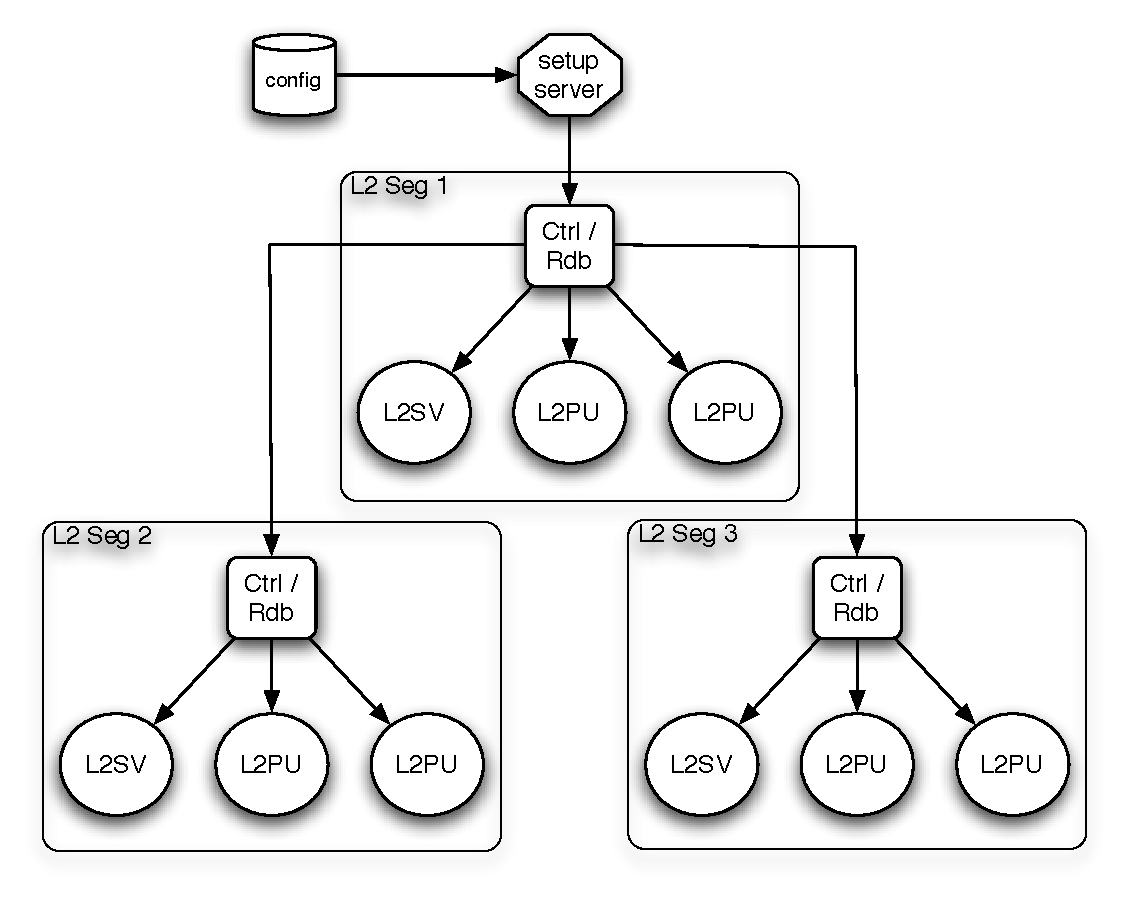
\includegraphics[width=0.6\textwidth]{oks_multi_control_strategy}
\caption{Estrutura de controle hierárquico do sistema de filtragem.}
\label{fig:multi_control}
\end{center}
\end{figure}

Para garantir sua escalabilidade, o sistema de filtragem pode ser dividido, logicamente, em \emph{segmentos}. Cada segmento contém sempre um controlador responsável por gerir os aplicativos dentro daquele segmento. Adicionalmente, utilizam-se múltiplos servidores de configuração, para evitar gargalos durante a fase de configuração. É apresentado, na Fig.~\ref{fig:multi_control}, um exemplo desta abordagem de controle hierárquico através da utilização de múltiplos segmentos. Como se percebe, ao multiplicar-se o número de aplicações de controle, diminui-se a carga de operações em cada controlador, permitindo que o número de aplicações aumente indefinidamente.  

Para a geração da base de dados de configuração, bem como a leitura da mesma, o ambiente OKS oferece interfaces de acesso em C++. Desta forma, o usuário fica isento dos detalhes de implementação e de localização da base de dados (local ou remota). Entretanto, a tarefa de configurar cada objeto, bem como a relação entre eles e sua organização lógica em segmentos, ainda fica a cargo do usuário, o que representa uma tarefa bastante penosa e delicada, requerendo conhecimento especialista, nem sempre disponível.


\section{O \emph{PartitionMaker}}
\label{sec:pm}

No início do desenvolvimento do sistema de filtragem de alto nível, as partições de configuração eram criadas manualmente, visto que a partição é um arquivo texto contendo os objetos descritos em linguagem XML \cite{bib:xml}. Entretanto, esta solução tornou-se rapidamente inviável devido ao grande número de componentes a serem configurados.

A primeira abordagem automática para a criação de base de dados de configuração era baseada em \emph{templates}. Nesta abordagem, o código XML de um objeto de cada classe ficava descrito como um modelo em um arquivo texto. Apenas alguns parâmetros podiam ser configurados, e os demais tinham valores pré-fixados. O usuário era, então, obrigado a configurar todos os parâmetros variáveis, o que restringia a utilização da ferramenta apenas aos usuários experientes. A falta de testes de consistência dos valores configurados resultava em freqüentes execuções mal sucedidas do sistema de filtragem. Por fim, como a descrição de cada objeto estava fixada, qualquer mudança na classe de um dado objeto, ou na implementação da base de dados, inutilizava a ferramenta de configuração até que o desenvolvedor da mesma atualizasse a sua base de \emph{templates}.

\begin{figure}
\begin{center}
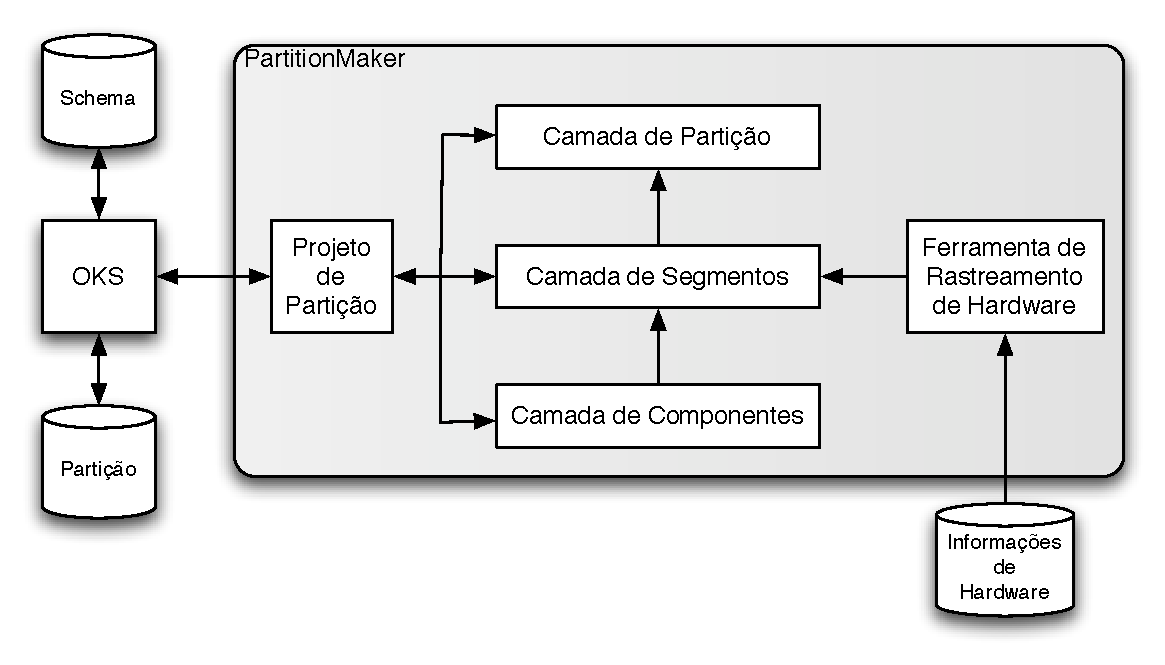
\includegraphics[width=0.65\textwidth]{partitionmaker_block_diagram}
\caption{Diagrama em blocos do \emph{PartitionMaker}.}
\label{fig:pm}
\end{center}
\end{figure}

Para se obter configuração automatizada, superando as falhas observadas nas abordagens anteriores, o \emph{PartitionMaker}, cujo diagrama é apresentado na Fig.~\ref{fig:pm}, foi desenvolvido. A filosofia deste ambiente é agregar o conhecimento especialista a respeito do sistema de filtragem, de forma que os usuários com diferentes níveis de conhecimento sobre o sistema de filtragem possam ser conduzidos com segurança durante o processo de configuração, resultando em execuções otimizadas e minimizando as possibilidades de erros. Por fim, o ambiente deve operar integrado à base de dados OKS, de forma a garantir que mudanças ocorridas na classe de um dado objeto sejam imediatamente reconhecidas pelo \emph{PartitionMaker}.

Ao ser inicializado pelo usuário, o \emph{PartitionMaker} lê a base de dados de \emph{schema} e gera uma representação em \emph{Python} \cite{bib:python} de cada uma das classes existentes. Esta leitura é realizada utilizando \emph{bindings} de C++ para Python \cite{bib:boost}, permitindo que o \emph{PartitionMaker} usufrua dos recursos já implementados na base de dados OKS, além de isentar o \emph{PartitionMaker} dos detalhes de implementação da base de dados de configuração e \emph{schema}. Toda esta operação de comunicação com o OKS é realizada pelo módulo de  \emph{Projeto de Partição}, de forma a abstrair do resto do sistema os detalhes desta comunicação.

\begin{figure}[t]
\begin{center}
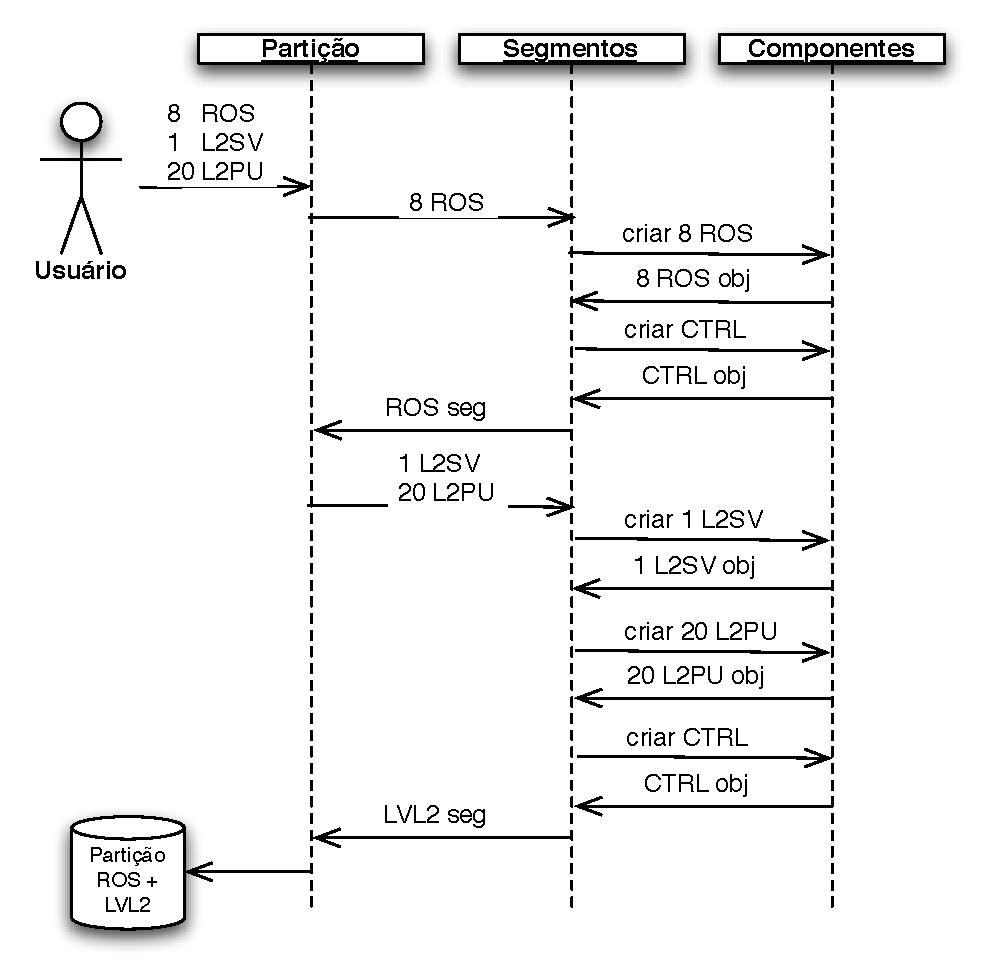
\includegraphics[width=0.6\textwidth]{partitionmaker_generation_flow}
\caption{Exemplo de fluxo de geração de uma partição.}
\label{fig:pm_flow}
\end{center}
\end{figure}

Após a inicialização, o usuário recorre aos diversos módulos e funções disponíveis, para atingir seus objetivos de configuração. De forma a atender uma vasta gama de usuários, com diferentes graus de familiaridade com o sistema de filtragem, uma abordagem em três camadas foi utilizada.

A camada mais baixa (\emph{Camada de Componentes}) é responsável por configurar cada objeto OKS individualmente. O controle de consistência, nesta camada, restringe-se a verificar se os limites aceitáveis para determinados atributos, tipo de dado inserido, entre outros, fazem sentido. Os objetos OKS são criados utilizando-se as funções da  base de dados OKS, evitando a replicação de código.

A segunda camada (\emph{Camada de Segmentos}) responsabiliza-se por acessar os objetos configurados pela primeira e agrupá-los na forma de segmentos com significado lógico para o sistema de filtragem. É de responsabilidade desta camada assegurar que as relações entre as aplicações dentro de um mesmo segmento estejam corretas, e que as aplicações contidas no mesmo apresentam relações entre si (por exemplo, evitando que uma aplicação do filtro de eventos esteja presente em um segmento destinado ao segundo nível). 

A última camada (\emph{Camada de Partição}) se encarrega de agrupar os segmentos gerados em uma base final de configuração, chamada de \emph{partição}, podendo esta ser finalmente utilizada para executar o sistema de filtragem. Nesta camada, é verificada se a relação entre segmentos está correta, para que os mesmos operem em harmonia.

Com esta abordagem multi-camada, usuários mais inexperientes com o ambiente e o sistema de filtragem podem trabalhar apenas na camada superior, de forma que, ao fornecerem poucos parâmetros gerais (número de processadores a serem utilizados, quais níveis devem ser executados, etc), o \emph{PartitionMaker} fornecerá uma base de configurações otimizada para os objetivos do usuário. Valores mais específicos são automaticamente calculados, graças ao conhecimento especialista agregado. Já usuários mais experientes, para atenderem casos de uso mais específicos, podem recorrer às camadas mais baixas do sistema. Usuários podem, inclusive, combinar recursos de várias camadas, por exemplo, gerando uma configuração padrão com a camada mais alta, e com recursos da camada mais baixa, alterar seus objetos e segmentos de acordo com suas necessidades especiais.

\begin{figure}[t]
\begin{center}
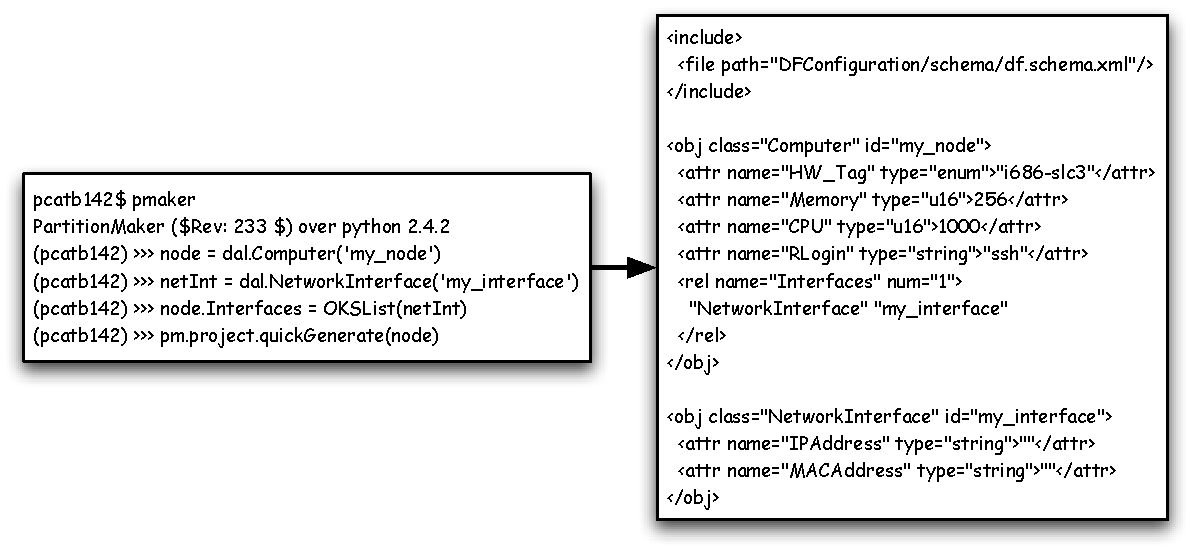
\includegraphics[width=0.7\textwidth]{ide}
\caption{Exemplo de geração de uma partição.}
\label{fig:ide}4
\end{center}
\end{figure}

É apresentado na Fig.~\ref{fig:pm_flow} um exemplo simplificado do fluxo de mensagens para a criação de uma partição contendo 8 ROS, além do LVL2 contendo 1 L2SV e 20 L2PU. No exemplo, o usuário trabalha somente com a camada mais alta. Ao especificar somente o número de componentes desejados, a camada de partição dispara mensagens para a camada de segmentos, de forma que sejam criados os segmentos para os ROS e LVL2. A camada de segmentos, por sua vez, ativa a camada de componentes, de forma que cada um dos objetos necessários sejam criados e retornados à camada de segmentos. Em seguida, a camada de segmentos agrupa tais componentes de maneira coerente à sua função, e os segmentos gerados são retornados para a camada de partição, para que sejam conectados e finalmente retornados ao usuário.

Outra etapa importante no processo de configuração é selecionar os nós de processamento a serem utilizados por cada aplicação. Para tal, o Módulo de Rastreamento de \emph{Hardware} permite rastrear um conjunto de máquinas de forma a analisar a propriedade destas (velocidade de \emph{clock}, quantidade de memória, interfaces de rede, etc), para melhor definir quais aplicações devem rodar em quais máquinas. Esta busca é feita em paralelo, através da utilização de várias \emph{threads} \cite{bib:modern_operating_systems} de execução, usando a estrutura de rede disponível. Isto resulta em tempos de busca bastante reduzidos, na ordem de poucas dezenas de segundos, para um conjunto de várias centenas de máquinas. 

Ao final deste processo de configuração, obtém-se uma representação da base de dados de configuração através de objetos em \emph{Python}. Esta base é então exportada, utilizando-se os recursos do módulo \emph{Projeto de Partição}, para o formato OKS de base de dados de configuração, podendo, finalmente, ser utilizada para a operação do sistema de filtragem de alto nível do ATLAS. Este módulo também permite que bases de dados de configuração já criadas possam ser importadas e editadas dentro do \emph{PartitionMaker}, proporcionando, desta maneira, que partições geradas com recursos externos ao \emph{PartitionMaker} também possam ser manipuladas neste ambiente.

Por ser implementado em \emph{Python}, o \emph{PartitionMaker} pode usufruir dos recursos bastante numerosos  desta linguagem. Como conseqüência, um ambiente integrado de desenvolvimento está disponível, permitindo rápida prototipagem de base de dados de configuração, conforme o exemplo na Fig.~\ref{fig:ide} demonstra. Ao inicializar o ambiente integrado, através do comando \texttt{pmaker}, o usuário acessa as funcionalidades do sistema. No exemplo, deseja-se configurar um nó de execução (\texttt{my\_node}) contendo uma interface de rede (\texttt{my\_interface}), usando, neste caso, a \emph{Camada de Componentes}. Ao final da configuração, os objetos criados em \emph{Python} são exportados para o formato utilizado pelo OKS através da função \texttt{quickGenerate}, cujo resultado aparece ao lado direito da Fig.~\ref{fig:ide}.

A facilidade da linguagem \emph{Python}, aliada ao ambiente integrado de desenvolvimento, permite que \emph{plugins} possam ser facilmente desenvolvidos para o \emph{PartitionMaker},  expandindo consideravelmente a capacidade do trabalho proposto. Por fim, como o ambiente integrado aceita comandos, tanto manualmente inseridos, bem como oriundos de um arquivo texto, \emph{scripts} de configuração podem ser escritos com facilidade, permitindo a execução de testes automáticos do sistema de filtragem do ATLAS, quando se deseja observar o comportamento deste sob diversas condições de operação (número de processadores, níveis de filtragem considerados, etc).

A abordagem utilizada para a concepção do \emph{PartitionMaker} resultou num claro aumento da produtividade dos desenvolvedores e operadores do sistema de filtragem do ATLAS. Antes, era necessária a presença de especialistas para garantir a correta configuração do sistema de filtragem. Com este conhecimento especialista embutido no \emph{PartitionMaker}, os usuários ficam mais independentes durante o processo de configuração. Isto resulta, também, em ganhos de produtividade para os técnicos especialistas, visto que minimiza-se a necessidade destes interromperem suas atividades para apoiar usuários menos experientes.

Outro resultado obtido foi a considerável diminuição de execuções mal sucedidas para os testes do sistema de filtragem do ATLAS. Com o \emph{PartitionMaker} identificando e notificando automaticamente possíveis erros durante a configuração, possíveis falhas podem ser identificadas antes da execução do sistema de filtragem, evitando-se a interrupção da operação do experimento.


\section{Automatic Online Triggering Execution}
\label{sec:runner}

Although the configuration process can be fully automated, by means of configuration database creation scripts, the execution of TDAQ is still manual. In order to start a given TDAQ run, once the configuration database is available, the following steps must be taken:

\begin{enumerate}

\item Boot: at this point the configuration database file is read, and the top level control applications are started. then, each control application starts up any controller placed beneath it within the segments hierarchy tree. After, each controller will start up any application within its segment, as well as all the configured RDB servers. All the applications are started up on the computer node designed for them in the database configuration file.

\item Configure: during this phase, the applications will retrieve their running configuration parameters from their RDB servers, which basically contain a cached copy of the original database configuration file. After this step, the TDAQ infrastructure is ready to begin its operation.

\item Run: this is the phase where data is actually being read from ATLAS detectors for the nominal use case, or from Monte Carlo simulation files if the TDAQ execution is envisaged for testing purposes. During this step, monitoring applications samples all TDAQ resources (memory consumption, LVL1 accept rate, CPU utilization, etc.), they also generate online histogramming with timing information, decision threshold achieved, etc. Finally, log files are created on the application nodes with any useful information for posterior analysis (warning / error messages issued, etc.). This running state is sustained until explicit user intervention requiring its interruption.

\end{enumerate}

While issuing the commands above manually is reasonable for the nominal operation case, it is quite tedious to perform all theses steps manually when several testing cases must be covered, which is a common case in the TDAQ development, either for TDAQ new releases validation and overnight tests, as well as for validation of new acquired hardware.

\begin{figure}
\begin{center}
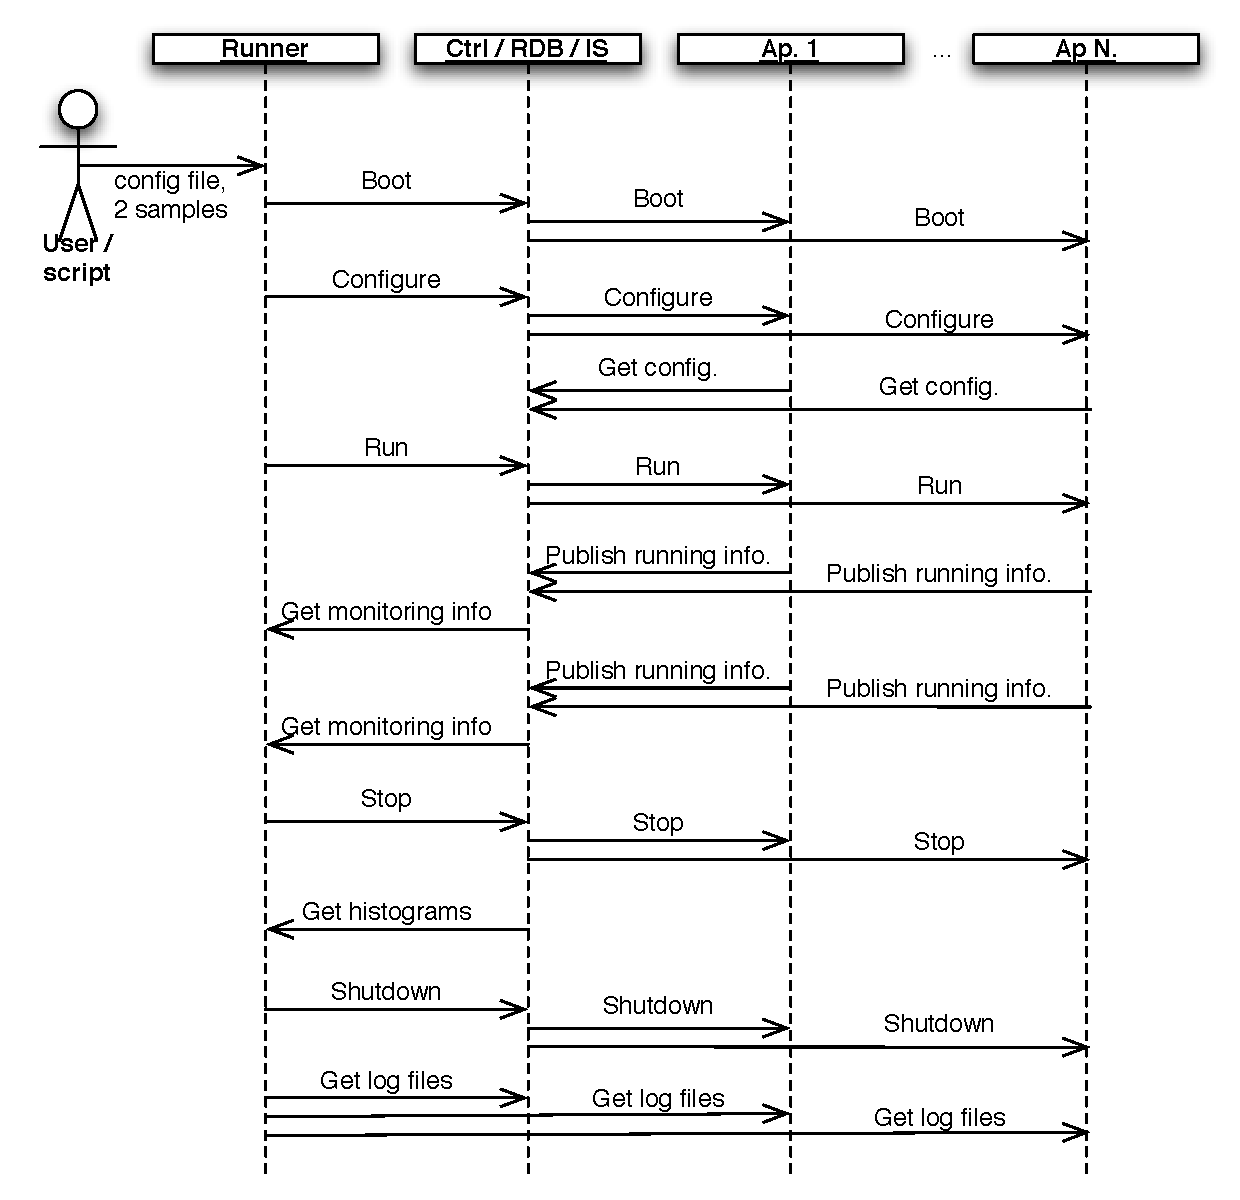
\includegraphics[width=0.6\textwidth]{runner_execution_flow}
\end{center}
\caption{Runner execution flow example.}
\label{fig:runner_exec_flow}
\end{figure}

Having this necessity in mind, the \emph{Runner} environment was developed. Its main goal is to provide an automated / scriptable way of running the TDAQ infrastructure, as well as collecting its monitoring information from the monitoring applications providing, if desired, a summarized report of the overall TDAQ execution. In Fig.~\ref{fig:runner_exec_flow} is presented a general example of the \emph{Runner} execution flow. In this example, the user (a running script, for instance) provides the configuration database file, and requests the TDAQ infrastructure to be executed for a time long enough so that 2 monitoring samples can be obtained. First the \emph{Runner} sends the message to the controller to boot the TDAQ modules to be used for this particular run. The controller then propagates the boot command to the rest of the applications. Next, the same sequence takes place, but this time to ask each TDAQ application to retrieve their configuration from the RDB server. In the next step, the \emph{Runner} asks the controller to send the command to start TDAQ operation. After that, each application will publish their monitoring information on their IS server, which is the application responsible for storing monitoring information. By knowing the monitoring sampling period, the \emph{Runner} can request the monitoring information published on the IS server. In the mean time, the online histogramming are being filled by the IS server. Once the 2 monitoring samples are collected, the \emph{Runner} issues the stop command to the controller, which propagates the command to all TDAQ applications. After, the online histograms are retrieved from the IS server, and the TDAQ infrastructure is requested to be shutdown. After this step, the \emph{Runner} connects to each of the nodes used in this TDAQ run to collect their log files. At the end, the monitoring information, log files and online histograms are returned to the user for further analysis, if desired.

The \emph{Runner} is presented as a set of Python modules. Therefore, the same IDE and syntax language available for the \emph{PartitionMaker} are available for the \emph{Runner}.  Consequently, plugins and running scripts can be easily developed for this environment. By combining these 2 environments, with an analysis framework with a Python interface, like ROOT \cite{bib:root}, the configuration, execution and analysis of the data obtained during TDAQ execution can be fully automated, greatly improving validation capabilities of the overall TDAQ infrastructure.



\chapter{Análise dos Eventos de Calorimetria}
\label{chap:dados}

Neste capítulo, serão apresentados os conjunto de dados utilizados para o desenvolvimento da pesquisa proposta. Adicionalmente, serão apresentadas as técnicas utilizadas para o pré-processamento inicial destes dados, antes de serem efetivamente utilizados para estudo. Estudos serão apresentados para identificar as principais características dos eventos a serem discriminados, bem como para validar que não apresentam problemas que inviabilizem sua utilização.

\section{Geração dos Eventos}
\label{sec:geracao_eventos}

Os eventos utilizados neste trabalho são oriundos de simulações de Monte Carlo ***REF*** produzidas pelos próprios colaboradores do ATLAS utilizando o \emph{Pythia} e o \emph{Geant}, e que ficam disponíveis para análise. ***FALAR O QUE TEM NESSES DADOS (PRE-FILTRADOS PELO LVL1, BYTE STREAM JA FEITO, OU SEJA, COMPARANDO COM A FAQUISICAO REAL DE DADOS, ESTES EVENTOS SIMULAM QUAL PONTO?)***. A tabela~\ref{tab:datasets} apresenta as informações dos conjuntos utilizados. São apresentados o nome de cada conjunto, conforme nomenclatura definida em ***REF***. 

\begin{table}
\caption{Informações dos eventos utilizados para análise.}
\begin{center}
{\tiny
\begin{tabular}{|l|l|l|l|l|}
\hline
\textbf{Conjunto} & \textbf{Tipo} & \textbf{\emph{Pile-up}} & \textbf{Energia (Gev)} & \textbf{Quantidade} \\
\hline
mc08.107020.singlepart\_e\_Et7-80.digit.RDO.e342\_s439 & Elétrons simples & Não & 7-80 & X \\
\hline
misal1\_mc12.005802.JF17\_pythia\_jet\_filter.digit.RDO.v12003105 & Di-jatos & Não & Y & X \\
\hline
ideal2\_mc12.005011.J2\_pythia\_jetjet.digit.RDO.v13003004 & Di-jatos & Não & Y & X \\
\hline
ideal2\_mc12.005012.J3\_pythia\_jetjet.digit.RDO.v13003004 & Di-jatos & Não & Y & X \\
\hline
\end{tabular}
}
\end{center}
\label{tab:datasets}
\end{table} 

Para o desenvolvimento de sistemas de filtragem elétron / jato para o segundo nível de filtragem do ATLAS, estes eventos precisam, inicialmente serem pré-filtrados pelo primeiro nível, para que os estudos sejam realizados somente nos eventos que, de fato, chegarão ao segundo nível. Para tal, utilizou-se o Athena para emular o primeiro nível de filtragem, para que este isolasse as regiões de interesse a serem propagadas ao segundo nível. Para que o conjunto resultante da filtragem contenha a maior quantidade possível de especificidades, um corte de baixa energia (7 Gev) foi utilizado, sendo este limiar de corte recomendado pela colaboração ATLAS para análises. Adicionalmente, o LVL1 foi configurado para não observar o vazamento de energia para a camada hadrônica (cortes sem isolamento). Desta maneira, o conjunto de RoI resultante conteria eventos de todas as assinaturas geradas pelo LVL1. Uma vez selecionadas,  as RoI foram copiadas para um arquivo em disco para que pudessem ser analisadas \emph{offline}. É apresentado na tabela~\ref{tab:num_eventos_filtrados}  o número final de regiões de interesse obtidas ao final do processo de pré-filtragem pelo LVL1\footnote{Os números apresentados são os totais por tipo de partícula, independente do conjunto de origem.}.

\begin{table}
\caption{Número de RoI obtidas para cada padrão após filtragem pelo LVL1.}
\begin{center}
\begin{tabular}{|l|l|}
\hline
\textbf{Padrão} & \textbf{Total de Eventos} \\
\hline
Elétron & 470.282 \\
\hline
Jato &  1.366.548 \\
\hline
\end{tabular}
\end{center}
\label{tab:num_eventos_filtrados}
\end{table} 

A figura~\ref{fig:estatistica_inicial}, são apresentados os histogramas de energia transversa total de cada RoI, além dos valores de $\eta$, $\phi$ e dos códigos dos detetores de cada célula. Para a distribuição de energia, consideramos apenas o espectro de energia na faixa de $7 \le E_T \le 80$ Gev, visto que é nesta região que se encontram as principais assinaturas de eventos eletromagnéticos. Para a distribuiçào em $\eta$, a análise desconsiderou a parte interna da tampa e o \emph{forward calorimeter}, visto que a probabilidade de eventos interessantes nesta região é bastante reduzida ***REF***.  No caso da distribuição em $\phi$, observa-se que  as células cobrem toda a faixa entre $\pm \pi$, permitindo a análise do peculiar caso onde o centro da RoI fica perto da região de $\pm \pi$ (\emph{phi-wraparound}). Por fim, a distribuição de células pelas camadas de cada calorímetro mostra que todos os subdetetores, com exceção do \emph{forward calorimeter} foram considerados. A linha tracejada apresentada indica qual seria o valor esperado do número de celulas em cada camada, considerando o tamanho de cada célula. Por exemplo, a primeira camada eletromagnética (\texttt{EM1}), na região do barril,  possui células cujo tamanho é a metade das células na segunda camada eletromagnética (\texttt{EM2}), para a mesma região,d e tal forma que devemos encontrar, aproximadamente o dobro do numero de células em (\texttt{EM1}) do que em (\texttt{EM2}), como confirma a figura~\ref{fig:estatistica_inicial}.

\begin{figure}
\centering 
\subfloat[Elétrons]{\label{fig:estatistica_inicial_eletrons} 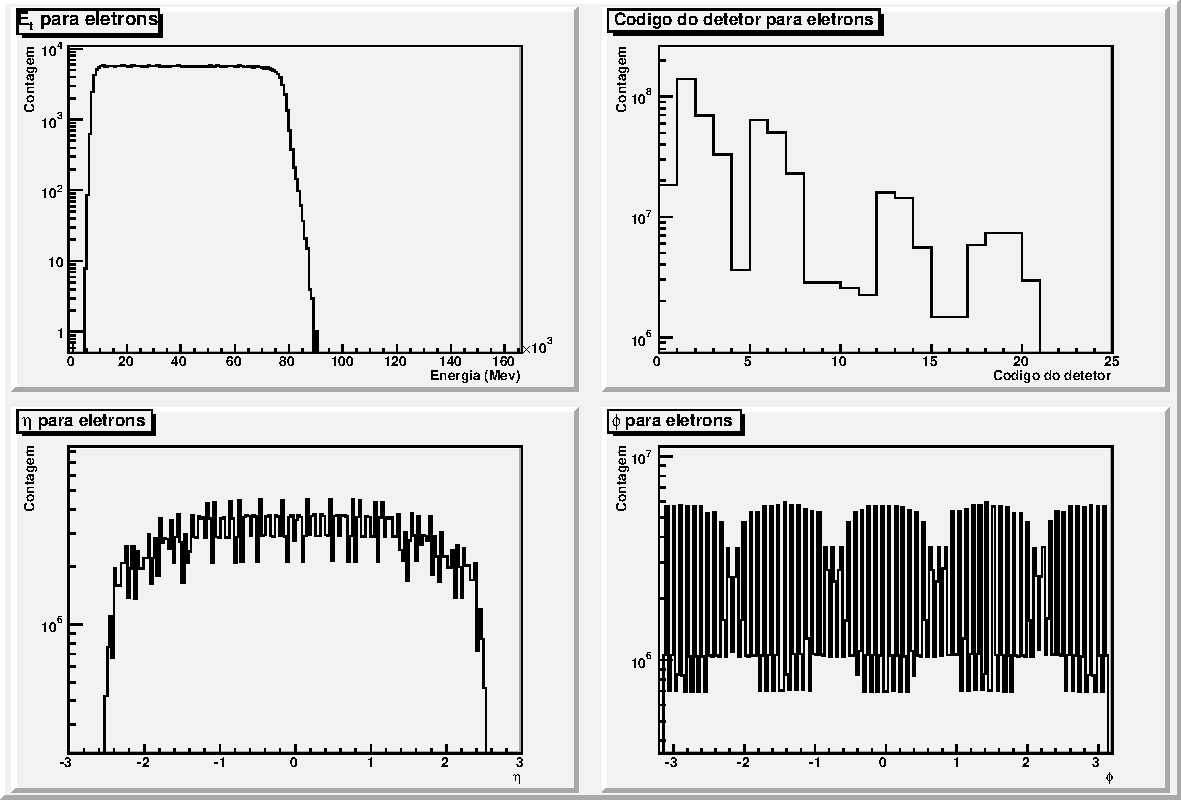
\includegraphics[height = 7cm]{hist_et_det_eta_phi_for_electrons}} \\
\subfloat[Jatos]{\label{fig:estatistica_inicial_jatos} 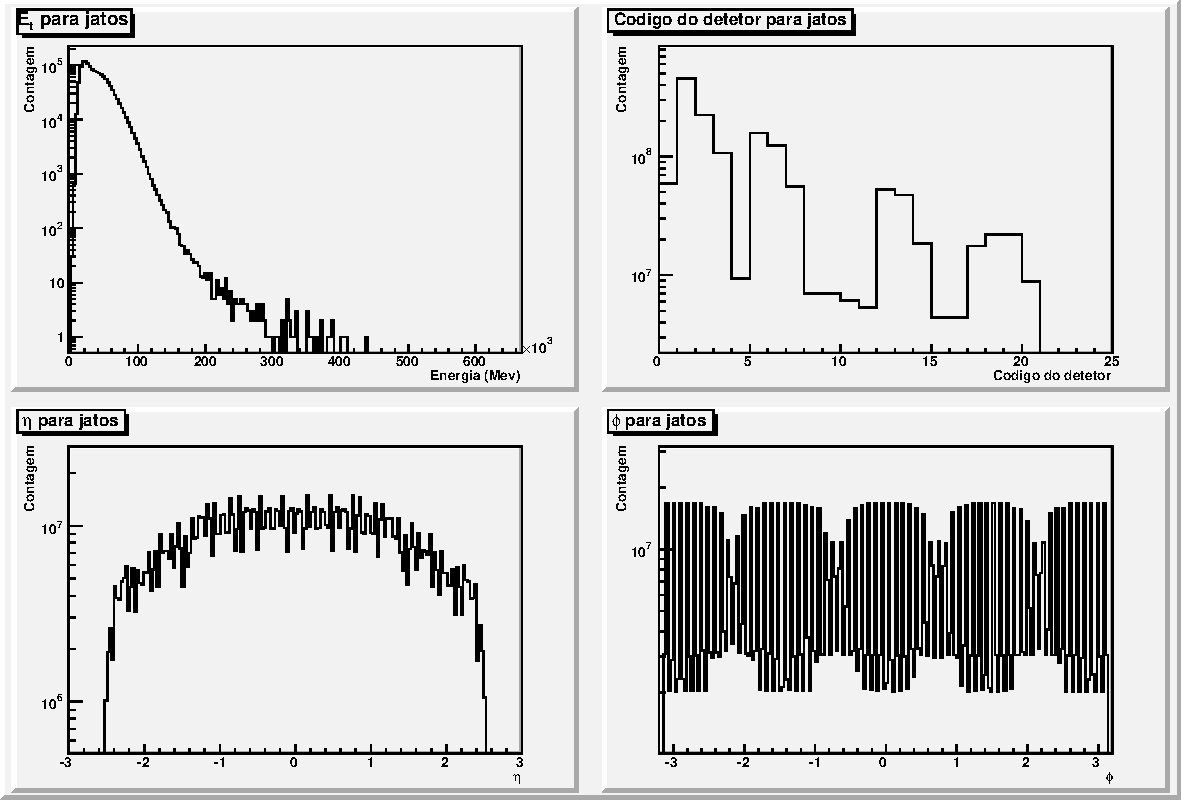
\includegraphics[height = 7cm]{hist_et_det_eta_phi_for_jets}}
\caption{Distribuição da informação proveniente dos calorímetros para cada tipo de partícula.} 
\label{fig:estatistica_inicial} 
\end{figure} 




 
\backmatter

%\nocite{*}
  
\bibliographystyle{coppe-unsrt}
\bibliography{bibliografia}

%\appendix
%\chapter{Codigo Fonte}

\end{document}
